% ----------------------------------------------------------
% Ajuda.Ai
% ----------------------------------------------------------
\chapter{Aplicativo Descubra Piauí} \label{cha:}

A metodologia utilizada neste trabalho tem como principal objetivo compreender de que maneira um aplicativo móvel pode contribuir para o desenvolvimento cultural local, por meio do mapeamento, do registro e da divulgação de pontos culturais acessíveis à população. O projeto surgiu da necessidade específica de valorizar a cultura do estado do Piauí e de oferecer uma ferramenta que fosse intuitiva, interativa e, acima de tudo, inclusiva, permitindo que tanto moradores quanto visitantes conheçam melhor os espaços turísticos e históricos da região.

Ao longo do desenvolvimento, a solução evoluiu de um protótipo inicial para um sistema completo, estruturado na forma de arquitetura cliente-servidor. Nesse modelo, o Descubra Piauí passou a ser composto por um frontend desenvolvido em Flutter, capaz de atender tanto a dispositivos móveis quanto à web, e por um backend implementado em Node.js, exposto por meio de uma API REST responsável pelo consumo e pela persistência dos dados em um banco relacional. Essa divisão em camadas tornou possível separar de forma mais clara as responsabilidades de interface, lógica de apresentação e regras de negócio, além de facilitar a manutenção e futuras extensões da aplicação.

A pesquisa foi organizada em duas etapas principais, que se relacionam diretamente com essa evolução. A primeira etapa consistiu em uma revisão teórica e documental, abordando temas como cultura digital, geolocalização, acessibilidade e uso de aplicativos móveis como ferramenta de promoção cultural, os quais fundamentaram a definição dos requisitos do sistema. A segunda etapa envolveu o desenvolvimento prático do aplicativo, inicialmente em forma de protótipo com dados simulados, e posteriormente em uma versão integrada a um backend próprio, com autenticação, persistência em banco de dados e suporte a funcionalidades avançadas, como avaliações, comentários e favoritos associados aos pontos culturais.

O aplicativo foi projetado seguindo o padrão arquitetural Model-View-Controller (MVC), tanto no frontend em Flutter quanto na organização do backend, o que contribuiu para uma melhor organização do código e para a separação entre modelos de dados, controles de fluxo e camadas de apresentação. No frontend, essa estrutura é combinada com mecanismos de gerenciamento de estado, permitindo que a interface reaja de forma consistente às ações do usuário e às respostas retornadas pela API. No backend, a mesma preocupação se reflete na divisão entre rotas, controladores, serviços e camadas de acesso ao banco, garantindo um fluxo mais claro desde a requisição até a gravação dos dados.

Além disso, durante todo o processo de criação do Descubra Piauí, foram seguidos princípios de usabilidade e de inclusão digital, buscando construir uma interface simples, visualmente clara e fácil de navegar, sem abrir mão de recursos mais avançados. Entre eles, destacam-se o uso de mapas interativos, a extração de coordenadas a partir de links do Google Maps, a possibilidade de cadastro detalhado de informações (como horários de funcionamento, atividades e eventos relacionados aos pontos) e a adoção de mecanismos de segurança, como autenticação baseada em tokens, para proteger rotas administrativas e dados sensíveis. Dessa forma, o aplicativo consolida-se não apenas como um repositório de informações, mas como uma plataforma digital que apoia de maneira concreta o mapeamento e a valorização da cultura piauiense.


\section{Casos de Uso} \label{sec:casos}

Os casos de uso descritos nesta seção representam os principais fluxos de interação dos usuários com o aplicativo Descubra Piauí, contemplando desde o acesso básico às informações culturais até a gestão completa dos pontos cadastrados. Eles foram definidos considerando três perfis distintos de uso — visitante sem autenticação, usuário logado e administrador — de forma a organizar claramente quais ações são permitidas para cada tipo de acesso. Dessa maneira, a modelagem busca equilibrar abertura de consulta pública com mecanismos de participação e controle, preservando a segurança e a integridade dos dados culturais registrados no sistema.

\begin{lista}
  \item \textbf{Caso de Uso 01 - Cadastro de Ponto Cultural}: o administrador acessa a tela de cadastro e insere informações como cidade, zona, nome do local, descrição, imagens, localização geográfica via GPS ou inserção manual, além das opções de acessibilidade disponíveis para o ponto. Ao confirmar o formulário, o sistema valida os dados e registra o novo ponto, que passa a ser exibido no mapa e na lista de pontos culturais.
  
  \item \textbf{Caso de Uso 02 - Visualização de Pontos no Mapa}: o usuário acessa a tela do mapa interativo e visualiza marcadores correspondentes aos pontos cadastrados. Ao tocar em um marcador, o sistema exibe um resumo contendo nome, imagem representativa e um botão que permite acessar a tela com mais detalhes sobre o ponto cultural selecionado.
  
  \item \textbf{Caso de Uso 03 - Filtro e Busca de Pontos}: o usuário utiliza a barra de busca ou os filtros disponíveis para localizar pontos de interesse por cidade, zona ou termos textuais. O sistema processa os critérios informados e retorna uma lista contendo apenas os pontos que atendem aos filtros, facilitando a navegação em cenários com grande quantidade de registros.
  
  \item \textbf{Caso de Uso 04 - Consulta Detalhada de Ponto}: ao selecionar um ponto na lista ou no mapa, o usuário é direcionado para uma tela de detalhes que apresenta galeria de imagens, descrição completa, informações de localização e opções de acessibilidade presentes no local. Essa visão detalhada permite conhecer melhor as características do ponto cultural antes de uma possível visita.
  
  \item \textbf{Caso de Uso 05 - Interação com Pontos (Favoritos, Avaliações e Comentários)}: o usuário autenticado acessa a tela de detalhes de um ponto cultural e pode marcá-lo como favorito, registrar uma avaliação em estrelas e adicionar comentários. O sistema associa essas interações ao perfil do usuário e atualiza informações agregadas, como a média das avaliações e a lista de comentários exibidos para todos os demais usuários.
  
  \item \textbf{Caso de Uso 06 - Administração de Estrutura e Informações Complementares}: o administrador gerencia cidades, zonas e dados complementares dos pontos culturais, como horários de funcionamento, atividades permanentes e eventos vinculados. Por meio de telas específicas, é possível criar, editar ou remover esses registros, garantindo que o conteúdo exibido no aplicativo permaneça organizado, atualizado e coerente com a realidade dos espaços culturais do estado.
\end{lista}

%As especificações dos casos de uso estão disponíveis no Anexo \ref{anexo:b} - Especificação de Casos de Uso. Apesar de outros casos de uso existirem, por serem bastante simples e triviais, como \emph{login}, \emph{logout}, CRUD simples de entidades do projeto \codigo{model} (apresentado no item \ref{sec:ajudaai:organizacao}) eles não foram documentados. Esses casos de uso são inclusos no diagrama de Casos de Uso, ilustrado na Figura \ref{fig:uml_caso_uso}. Como trabalho futuro, pretende-se implementar a Caso de Uso 03, pois atualmente os próprios \emph{Gateways} disponibilizam ferramentas dessa natureza.

% \begin{figure}[H]
%   \caption{\label{fig:uml_caso_uso}Diagrama UML de Casos de Uso do Ajuda.Ai}
%   \centering
%   \includegraphics[scale=0.5]{imagens/uml-casos-de-uso-03.pdf}
%   \legend{Fonte: Elaborado pelo Autor}
% \end{figure}

A seguir serão apresentados detalhes sobre a implementação do projeto, como tecnologias utilizadas, e em seguida uma apresentação visual da aplicação criada. 


\section{Características da Implementação} \label{sec:caracteristicas}

A implementação do Descubra Piauí foi organizada seguindo uma arquitetura em camadas, baseada no padrão Model-View-Controller (MVC) e na separação entre cliente e servidor. O sistema é composto por um frontend desenvolvido em Flutter, voltado tanto para dispositivos móveis quanto para web, e por um backend implementado em Node.js, exposto por meio de uma API REST que realiza a comunicação com o banco de dados relacional. Essa abordagem favorece a modularidade, a manutenção e a possibilidade de evoluir cada parte da solução de forma independente.

\subsection{Frontend em Flutter}

No frontend, o projeto foi estruturado em módulos de \textit{models}, \textit{views}, \textit{controllers} e \textit{repositories}, alinhados ao padrão MVC. As classes de modelo representam entidades como \textit{Usuário}, \textit{Cidade}, \textit{Zona}, \textit{PontoInteresse}, \textit{Acessibilidade} e demais elementos que compõem a estrutura cultural mapeada pelo aplicativo. As \textit{views} correspondem às telas do sistema, incluindo mapa interativo, lista de pontos, detalhes, formulários de cadastro e telas de autenticação, todas construídas com foco em clareza visual e navegação simples para o usuário final.

Os \textit{controllers}, em conjunto com o pacote \texttt{provider} e a interface \texttt{ChangeNotifier}, são responsáveis pelo gerenciamento de estado e pela orquestração das interações entre interface e dados. Por meio desse mecanismo, a aplicação consegue reagir às ações do usuário e às respostas da API de forma reativa, atualizando a interface sempre que ocorre alguma mudança relevante no estado. Já os \textit{repositories} encapsulam a comunicação HTTP com o backend, utilizando a biblioteca \texttt{Dio} para definição de endpoints, tratamento de erros, envio de tokens de autenticação e conversão de estruturas JSON para os modelos internos do aplicativo.

Além disso, foram integrados recursos específicos para atender às necessidades do projeto. A biblioteca \texttt{FlutterMap}, em conjunto com os tiles do OpenStreetMap, é utilizada para exibir o mapa interativo com os pontos culturais distribuídos no território. A obtenção de coordenadas geográficas é realizada com apoio da \texttt{geolocator}, enquanto a compressão de imagens antes do envio é feita por meio de \texttt{flutter\_image\_compress}, reduzindo o consumo de banda e de armazenamento. A persistência local do token JWT ocorre com \texttt{SharedPreferences}, permitindo que o usuário permaneça autenticado entre sessões sem necessidade de refazer o login a cada abertura do aplicativo.

\subsection{Backend em Node.js e Banco de Dados}

No backend, a aplicação foi construída em Node.js utilizando o framework \texttt{Express} para organização das rotas e controladores da API REST. As rotas definem os caminhos para operações relacionadas a autenticação, cidades, zonas, pontos de interesse, favoritos, avaliações, comentários, horários, atividades e eventos, seguindo uma convenção de métodos HTTP (\texttt{GET}, \texttt{POST}, \texttt{PUT}, \texttt{DELETE}) coerente com cada tipo de operação. Os controladores recebem as requisições, validam os dados de entrada e delegam o processamento às camadas de serviço.

As regras de negócio são centralizadas em serviços, responsáveis por tarefas como cadastro de novos pontos, atualização de informações, associação de favoritos a usuários, cálculo de médias de avaliação e vinculação de atividades e eventos a cada local. O acesso ao banco de dados é realizado por meio do \textit{ORM} \texttt{Prisma}, que mapeia as entidades da aplicação para tabelas em um banco PostgreSQL. Essa abordagem facilita a definição do esquema de dados, o versionamento de alterações por \textit{migrations} e a execução de consultas tipadas, reduzindo erros comuns de acesso direto ao banco.

A infraestrutura de dados e armazenamento contempla o uso do Supabase tanto para hospedagem do banco PostgreSQL quanto para o \textit{storage} de imagens associadas aos pontos culturais. Com isso, o backend passa a ser responsável apenas pela lógica de negócio e pela integração com esses serviços externos, enquanto o gerenciamento de arquivos e da instância de banco é delegado à plataforma. O deploy do backend em ambiente de produção é realizado em serviços de nuvem, como o Koyeb, permitindo que a API fique disponível de forma pública e escalável para ser consumida pelo frontend.

\subsection{Modelagem de Dados}

A modelagem de dados do Descubra Piauí foi construída de forma a representar, de maneira organizada, os principais elementos envolvidos no mapeamento cultural do estado. No núcleo da estrutura está a entidade \textit{PontoInteresse}, que representa cada ponto cultural, histórico ou turístico cadastrado no sistema. A ela estão associadas informações como localização geográfica, descrição textual, imagens ilustrativas e opções de acessibilidade disponíveis no local.

Do ponto de vista geográfico, cada \textit{PontoInteresse} está vinculado a uma \textit{Zona}, que, por sua vez, pertence a uma \textit{Cidade}. Essa hierarquia (\textit{Cidade} $\rightarrow$ \textit{Zona} $\rightarrow$ \textit{PontoInteresse}) facilita a organização dos dados e sustenta os filtros utilizados na interface, permitindo que o usuário pesquise pontos por município e por região específica dentro desse município. Além disso, o modelo contempla entidades complementares relacionadas ao ponto, como \textit{Acessibilidade}, \textit{HorarioFuncionamento}, \textit{Atividade} e \textit{Evento}, que armazenam informações sobre condições de acesso, horários de visitação e programações culturais associadas.

Em relação aos usuários, a entidade \textit{Usuario} mantém os dados de identificação e autenticação, além de se relacionar com outros registros que representam sua interação com os pontos culturais. Entre essas relações destacam-se \textit{Favorito}, \textit{Avaliacao} e \textit{Comentario}, que indicam, respectivamente, os pontos marcados como favoritos, as avaliações em estrelas atribuídas e os comentários textuais deixados pelos usuários. Essa modelagem permite registrar, de forma estruturada, o engajamento da comunidade com os espaços culturais, possibilitando análises futuras sobre interesses e percepção de qualidade dos locais mapeados.

Com base nessa estrutura, foi elaborado um diagrama entidade-relacionamento que sintetiza os relacionamentos entre as principais entidades do sistema, servindo como referência visual tanto para o desenvolvimento quanto para a documentação do projeto.

\begin{figure}[H]
	\caption{\label{fig:der_01}Diagrama Entidade-Relacionamento}
    \centering
    \includegraphics[width=\textwidth]{imagens/diagrama_casos_uso.png}
    \legend{Fonte: Elaborado pelo Autor}
\end{figure}

\subsection{Segurança e Autenticação}

A camada de segurança da aplicação combina diferentes mecanismos para proteger dados sensíveis e restringir o acesso a funcionalidades administrativas. A autenticação de usuários é baseada em JSON Web Tokens (JWT), emitidos após o processo de login bem-sucedido e enviados pelo cliente em cada requisição a rotas protegidas. \textit{Middlewares} específicos no backend verificam a presença e a validade desses tokens, garantindo que apenas usuários autenticados acessem operações como registro de favoritos, avaliações e comentários, enquanto rotas de administração exigem, adicionalmente, o perfil adequado.

As senhas dos usuários são armazenadas de forma protegida, utilizando a biblioteca \texttt{bcrypt} para geração de \textit{hashes} com \textit{salt}, o que dificulta ataques de força bruta e exposição direta das credenciais em caso de vazamento de dados. As configurações sensíveis, como chaves secretas de JWT, credenciais de acesso ao banco de dados e parâmetros de serviços externos, são mantidas em arquivos de variáveis de ambiente (\texttt{.env}), que não são versionados junto com o código-fonte. Além disso, as tabelas mantidas no Supabase utilizam políticas de Row Level Security (RLS), restringindo o acesso direto aos dados e assegurando que as operações de leitura e escrita ocorram apenas por meio da API autorizada.

\subsection{Usabilidade, Design e Responsividade}

Desde o início do desenvolvimento, houve uma preocupação em alinhar a solução aos princípios de usabilidade e inclusão digital. A identidade visual do Descubra Piauí foi inspirada nas cores da bandeira do estado, utilizando principalmente tons de verde, azul e branco, de modo a reforçar o vínculo simbólico com o território representado e facilitar a identificação do aplicativo pelos usuários locais. A aplicação adota conceitos do Material Design, com componentes padronizados, espaços em branco bem distribuídos e tipografia legível, contribuindo para uma experiência visual coerente em todas as telas.

O tema visual foi centralizado por meio de \texttt{ThemeData} e classes auxiliares responsáveis por definir paleta de cores, estilos de texto e parâmetros de componentes, o que simplifica a manutenção e garante consistência no uso de elementos gráficos. Do ponto de vista responsivo, as telas foram planejadas para se adaptar tanto a smartphones quanto a navegadores web, ajustando espaçamentos, tamanhos de fonte e organização de blocos de conteúdo conforme o tamanho da tela disponível. Dessa forma, o Descubra Piauí busca oferecer uma experiência de uso fluida, acessível e visualmente agradável, independentemente do dispositivo utilizado pelo usuário.

\subsection{Fluxo de Autenticação e Autorização}

O fluxo de autenticação do Descubra Piauí foi projetado para diferenciar claramente o acesso de visitantes, usuários autenticados e administradores, garantindo ao mesmo tempo segurança e simplicidade de uso. No frontend, o processo se inicia quando o usuário informa suas credenciais na tela de login. Essas informações são enviadas à API, que valida os dados no banco de dados e, em caso de sucesso, gera um token JSON Web Token (JWT) contendo a identificação do usuário e o seu perfil de acesso.

Esse token é retornado ao cliente e armazenado localmente por meio do
\textit{SharedPreferences}. Assim, o usuário pode permanecer autenticado entre
sessões, sem precisar refazer o login a cada abertura do aplicativo. A partir
desse momento, as requisições para rotas protegidas da API passam a incluir o
token no cabeçalho de autenticação. No backend, \textit{middlewares}
específicos verificam sua validade e extraem as informações de perfil.
Funcionalidades como favoritar pontos, registrar avaliações e adicionar
comentários exigem autenticação. Já operações administrativas, como cadastrar e
editar pontos, cidades e zonas, exigem também perfil de administrador.

Dessa forma, o fluxo de autenticação e autorização garante que operações sensíveis sejam realizadas apenas por usuários devidamente autorizados, ao mesmo tempo em que preserva o acesso público às funcionalidades de consulta e navegação pelo mapa cultural. Essa combinação de mecanismos contribui para a proteção dos dados do sistema e para a integridade das informações exibidas aos usuários.


\section{Apresentação da Aplicação} \label{sec:ajudaai:apresentacao}

Nesta seção, será apresentada a solução desenvolvida neste trabalho por meio de um protótipo inicial do aplicativo. A proposta é ilustrar, de forma clara, as principais telas e funcionalidades da aplicação.

A tela inicial do app é composta por um mapa interativo, que permite ao usuário visualizar os pontos culturais já cadastrados. Cada ponto é marcado no mapa, facilitando a identificação da localização exata. Logo abaixo do mapa, encontra-se uma barra de ações com dois botões principais que são:  Lista de Pontos, que leva o usuário para uma visualização em formato de lista dos locais cadastrados, permitindo o uso de filtros e ordenações; Perfil do Usuário, que direciona para uma área pessoal onde o usuário poderá editar seus dados e acompanhar suas contribuições no aplicativo.

Essa tela inicial foi pensada para oferecer uma navegação simples e direta, facilitando o acesso rápido tanto à visualização espacial quanto às informações detalhadas dos pontos culturais.

\begin{figure}[H]
	\caption{\label{fig:descubra_piaui_01}Captura de Tela da Página Inicial}
    \centering
    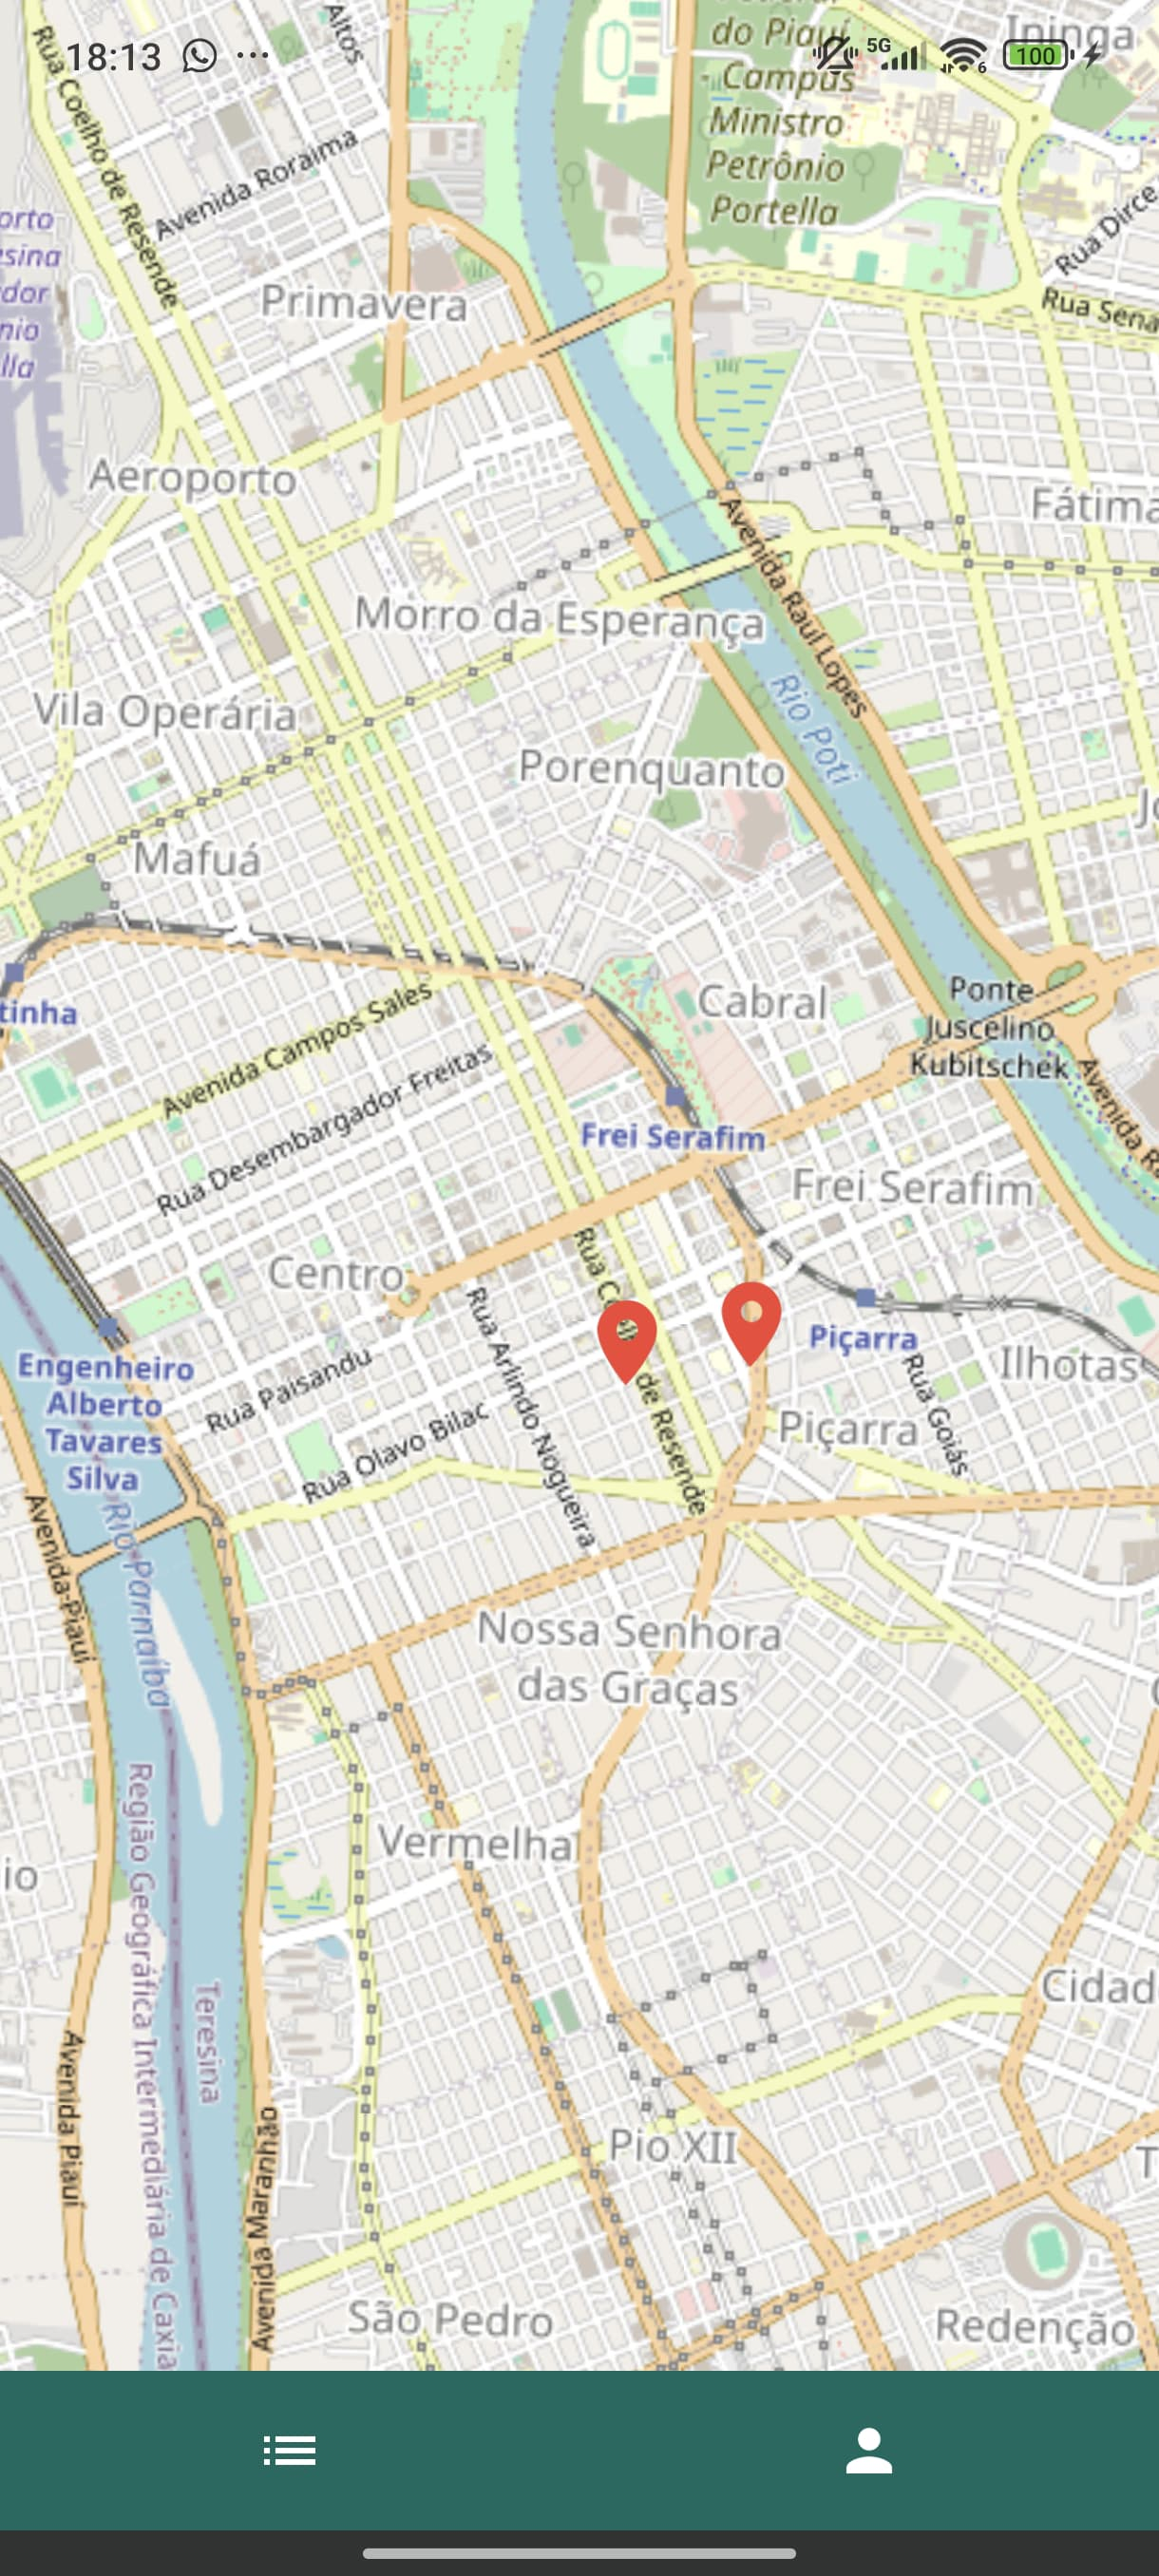
\includegraphics[scale=0.15]{imagens/tela_inicial.jpeg}
    \legend{Fonte: Elaborado pelo Autor}
\end{figure}

Na página Lista de Pontos, são exibidos todos os locais culturais que foram cadastrados no sistema. Essa funcionalidade permite ao usuário visualizar os pontos de forma organizada, facilitando a navegação e a busca por informações específicas.

O usuário pode percorrer a lista manualmente ou utilizar as ferramentas de busca disponíveis, como filtros por cidade, tipo de acessibilidade, ou palavra-chave. Essa interface foi desenvolvida para oferecer uma alternativa prática ao mapa interativo, especialmente para quem prefere pesquisar de forma direta por nomes ou categorias.

\begin{figure}[H]
	\caption{\label{fig:ss_ajudaai_02}Captura de Tela da Página de Lista de Pontos}
    \centering
    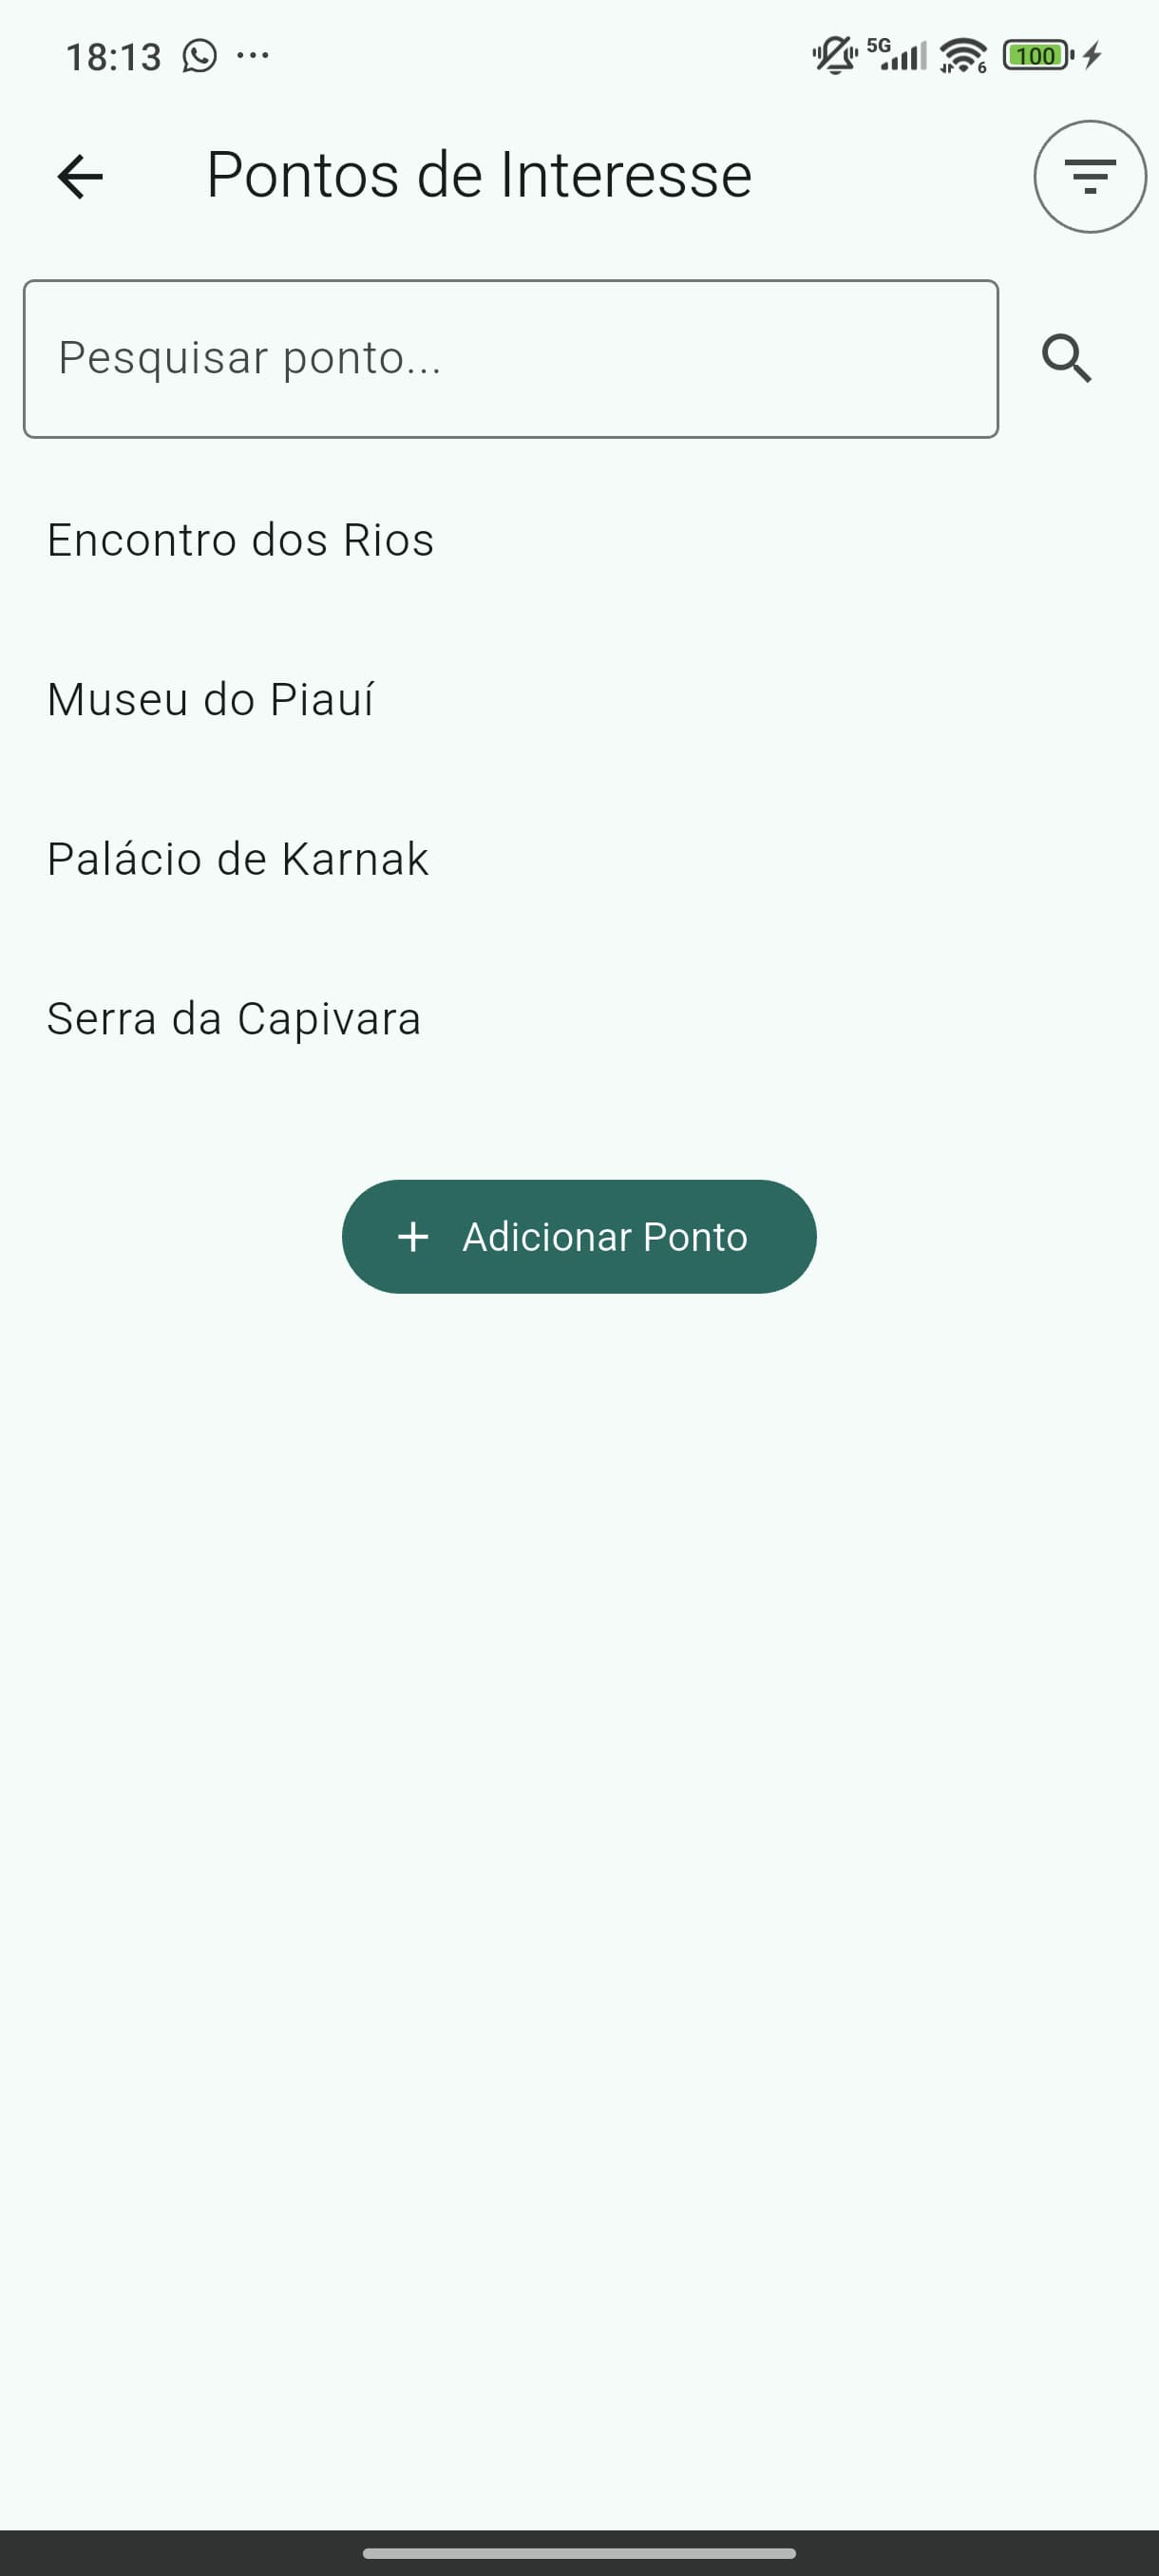
\includegraphics[scale=0.15]{imagens/lista_pontos.jpeg}
    \legend{Fonte: Elaborado pelo Autor}
\end{figure}

Entre as ferramentas disponíveis na tela Lista de Pontos, destaca-se o filtro de busca, que permite ao usuário localizar os pontos culturais de forma mais precisa. Essa funcionalidade possibilita a filtragem por cidade e zona, permitindo que o usuário visualize apenas os locais vinculados a uma determinada região geográfica.

Esse recurso foi pensado para facilitar a navegação, especialmente em contextos onde há um grande número de pontos cadastrados, tornando a busca mais rápida, organizada e eficiente para o usuário.

\begin{figure}[H]
	\caption{\label{fig:ss_ajudaai_03}Captura de Tela da Página Lista de Ponto Exemplo de Filtro}
    \centering
    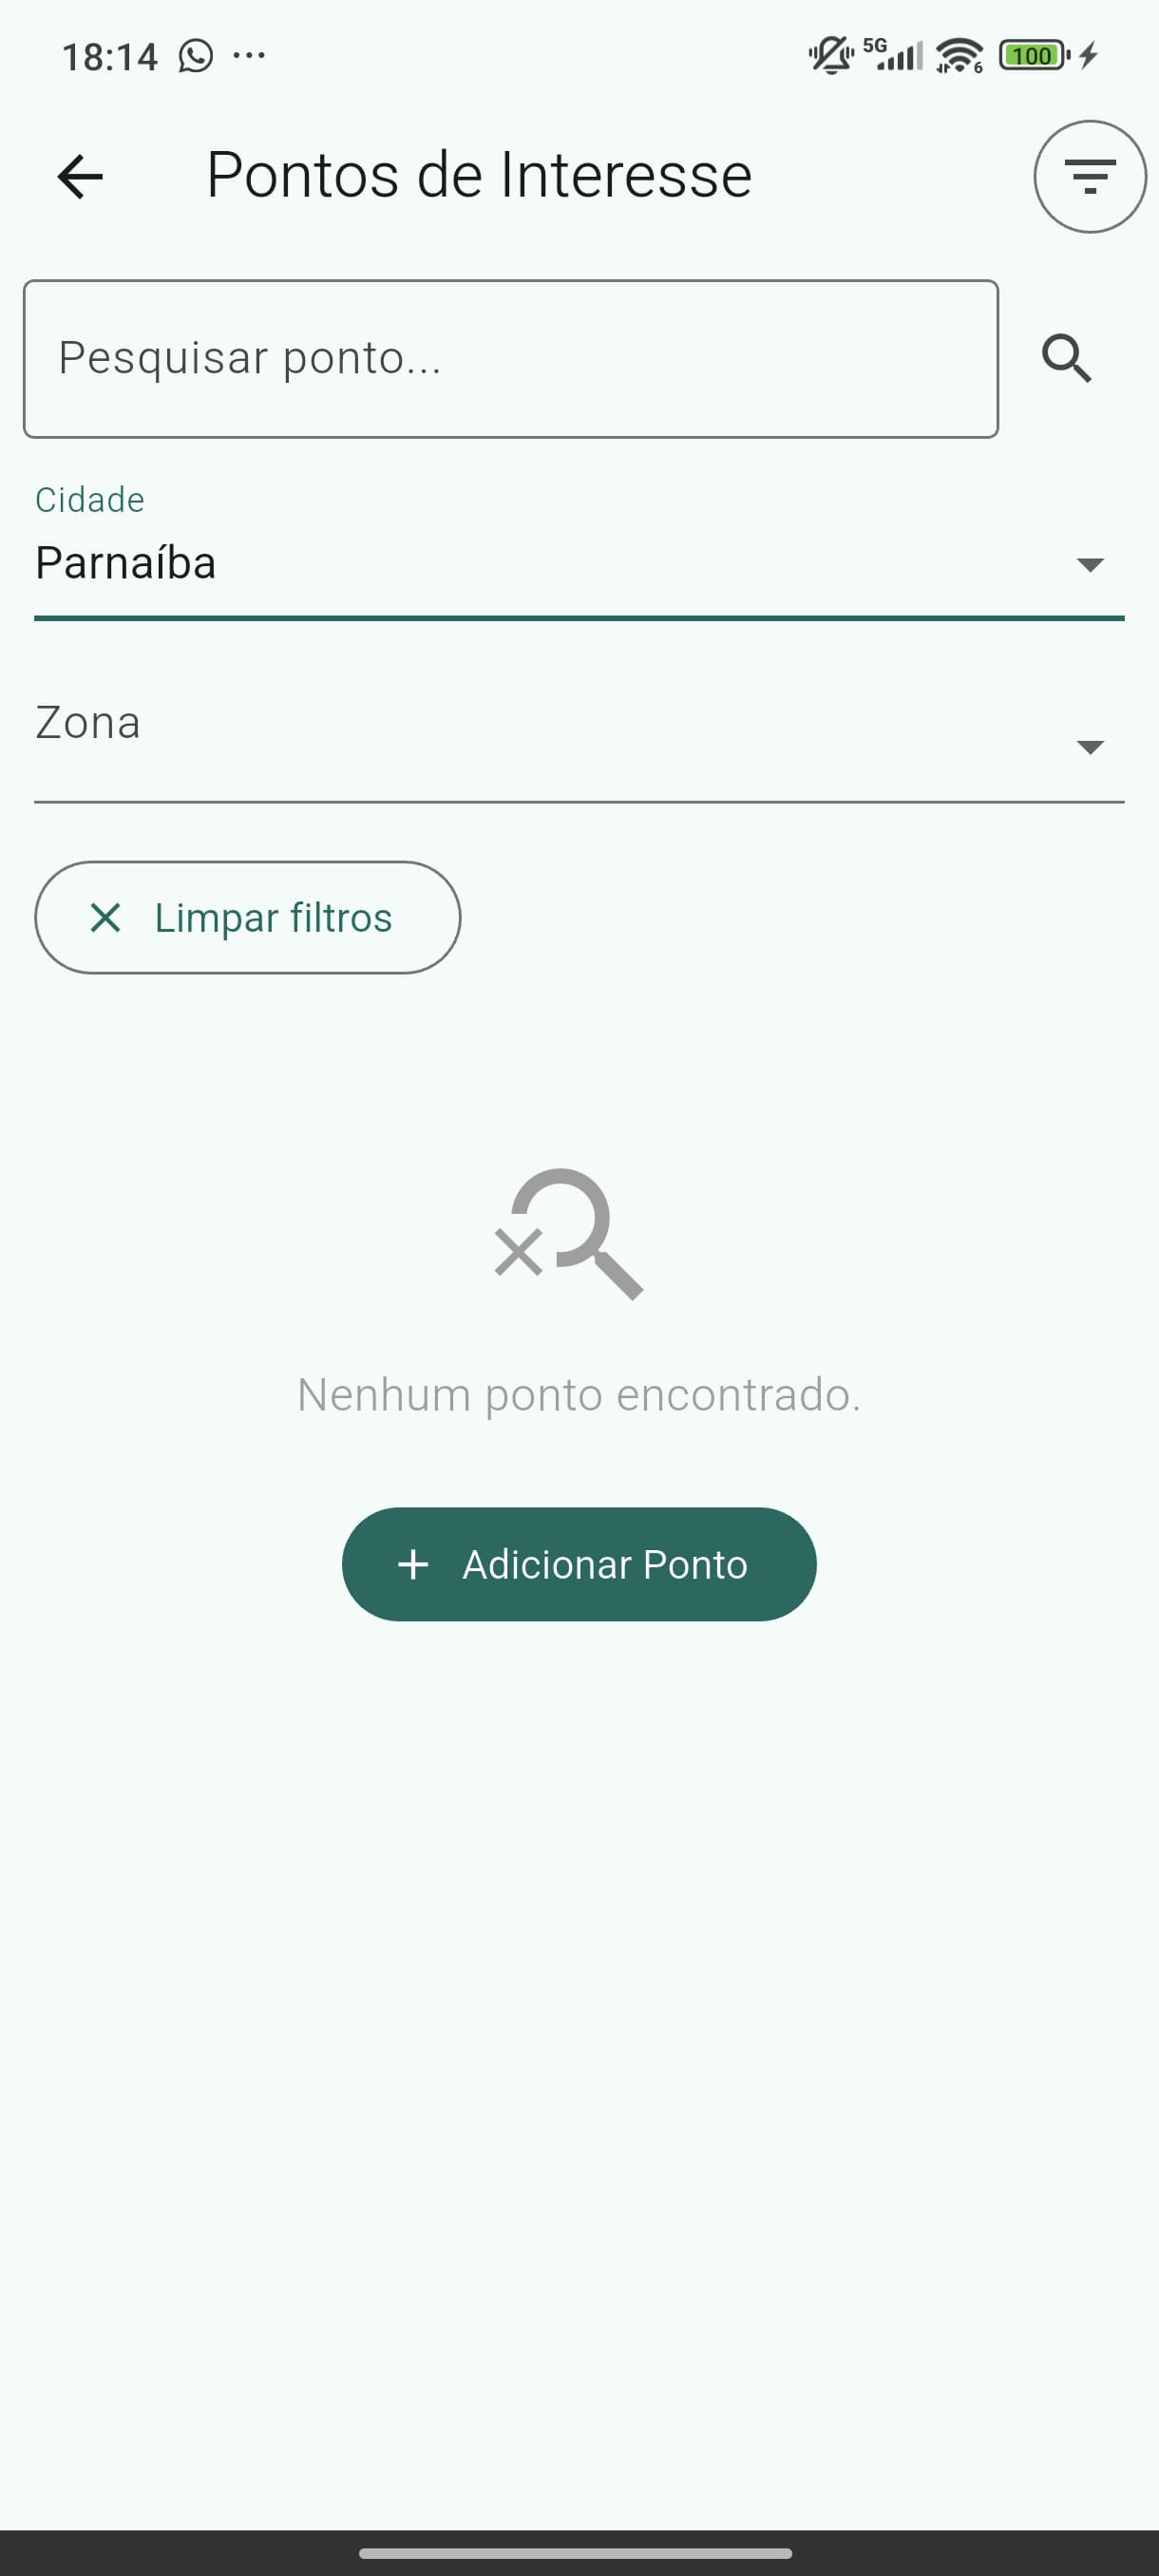
\includegraphics[scale=0.15]{imagens/filtros.jpeg}
    \legend{Fonte: Elaborado pelo Autor}
\end{figure}

Outra ferramenta disponível na tela Lista de Pontos é a barra de pesquisa textual, onde o usuário pode digitar diretamente o nome do ponto cultural que deseja localizar. Ao inserir o termo desejado, o sistema realiza a busca e exibe, de forma imediata, os resultados correspondentes.

Essa funcionalidade foi implementada para oferecer maior agilidade na localização de pontos específicos, otimizando a experiência do usuário e tornando a navegação mais objetiva e funcional.

\begin{figure}[H]
	\caption{\label{fig:ss_ajudaai_04}Captura de Tela da Página de Lista de Pontos Exemplo de Pesquisa}
    \centering
    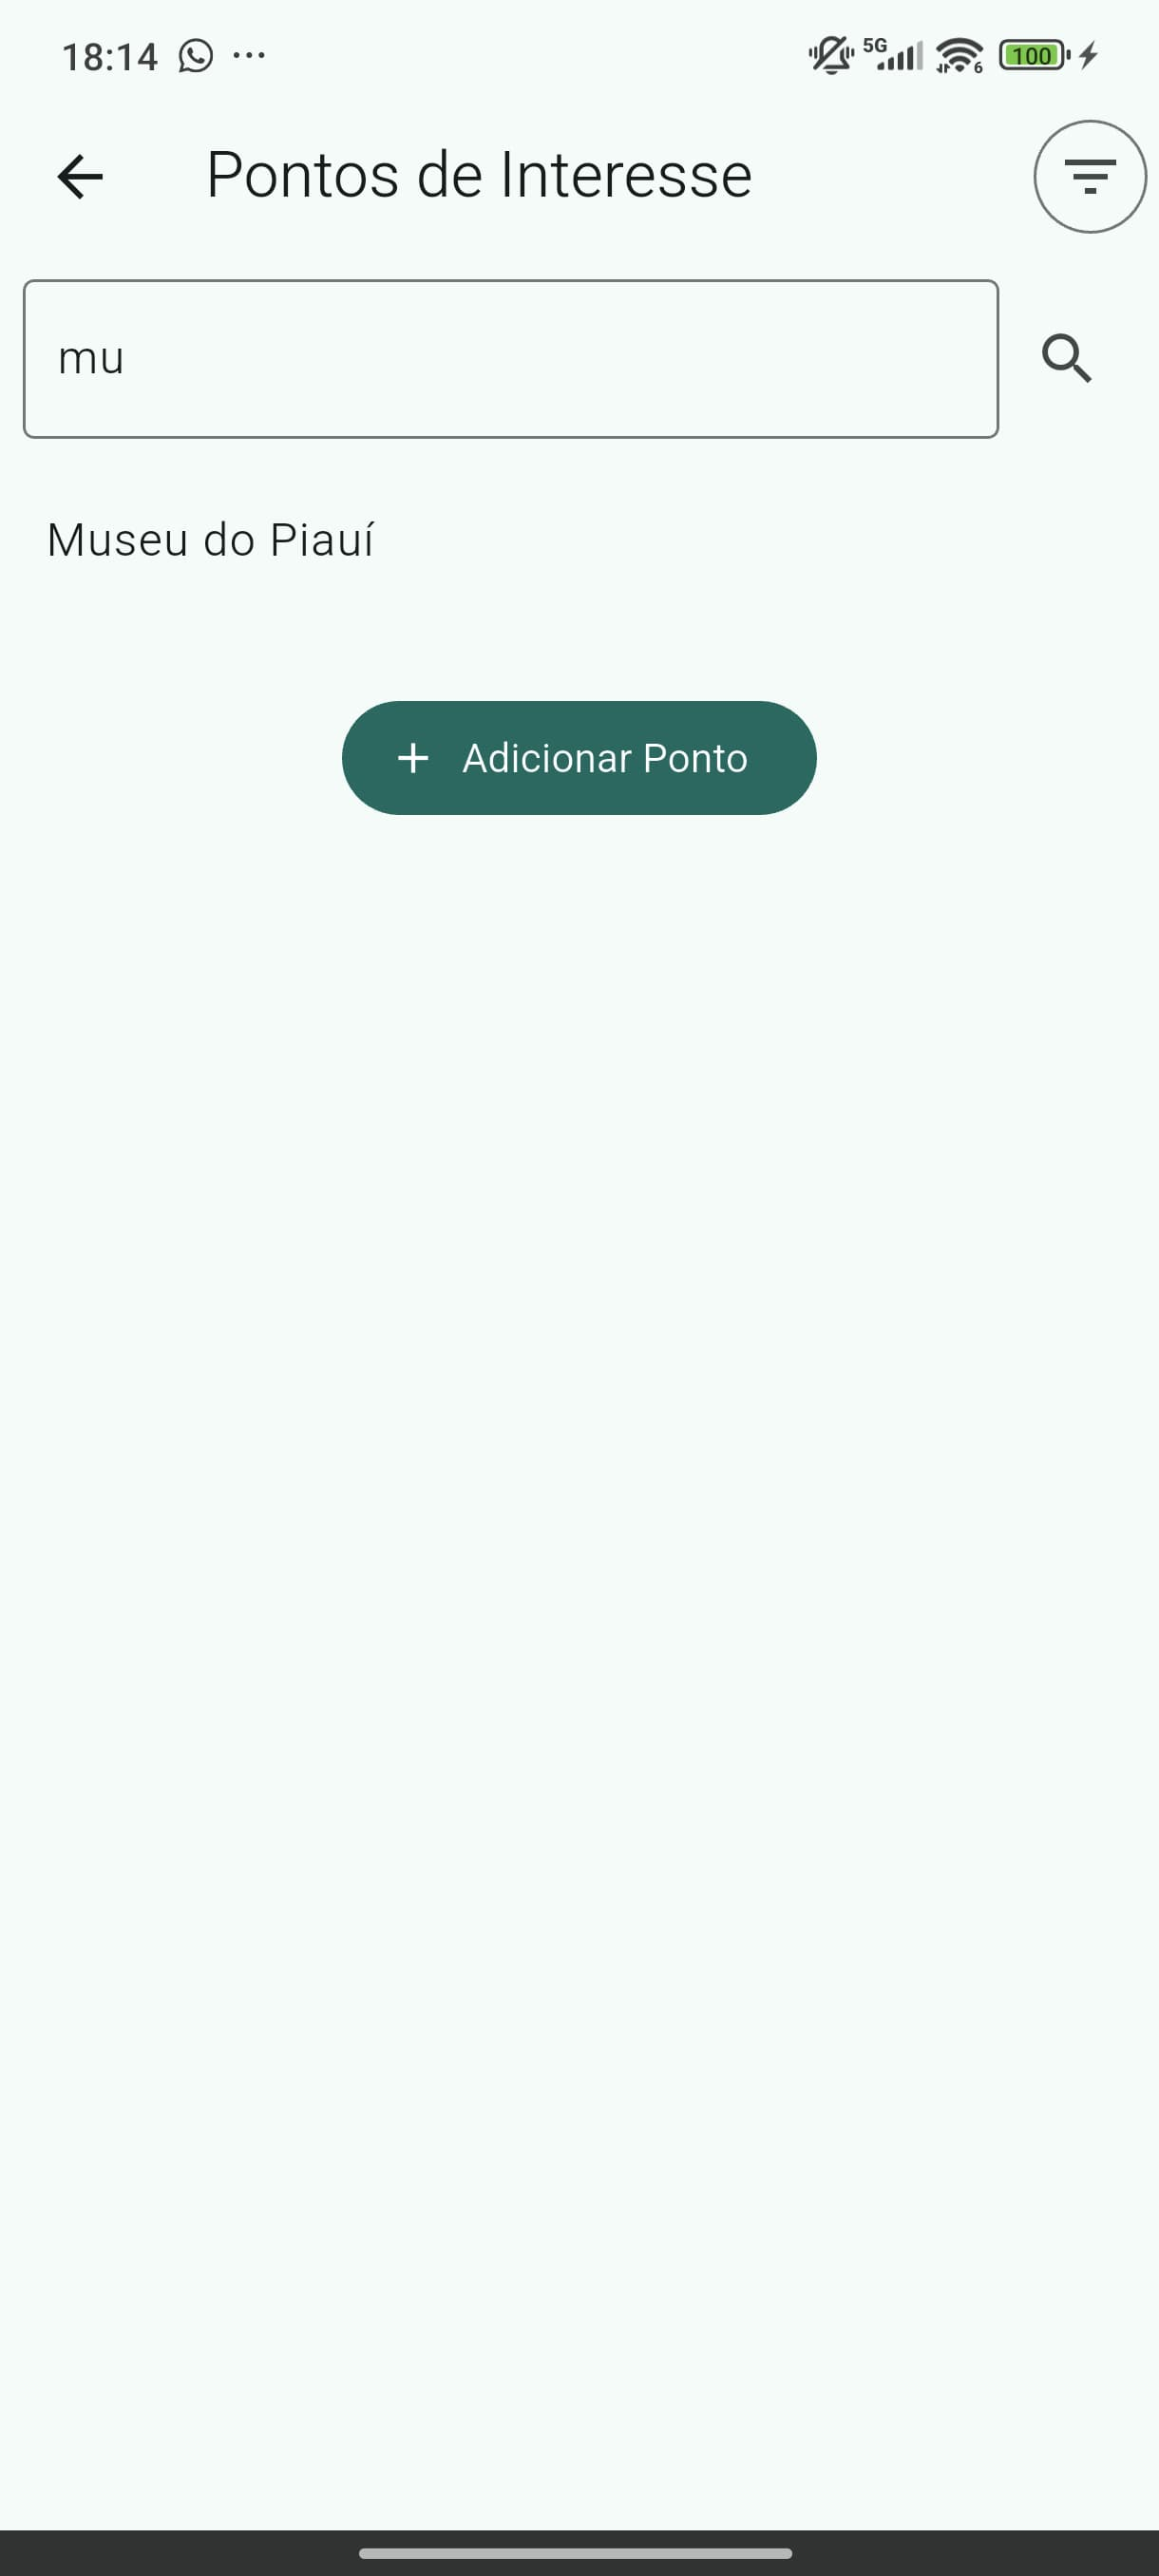
\includegraphics[scale=0.15]{imagens/pesquisa_ponto.jpeg}
    \legend{Fonte: Elaborado pelo Autor}
\end{figure}

A tela de adicionar ponto é uma das principais funcionalidades do sistema e está disponível exclusivamente para usuários com perfil de administrador. Nessa interface, é possível realizar o cadastro de novos pontos culturais por meio de um formulário composto por diversos campos.

O primeiro campo é o de cidade, que permite vincular o ponto a um município específico, facilitando a organização e futuras buscas. Caso a cidade desejada ainda não esteja cadastrada no sistema, há um botão logo abaixo do campo que possibilita adicionar uma nova cidade, conforme ilustrado na Figura 6.

Após a seleção da cidade, o campo de zona é habilitado. Ele exibe as zonas já cadastradas para aquela cidade, e também oferece a opção de adicionar uma nova zona, por meio de um botão específico logo abaixo, como mostrado na Figura 7.

Em seguida, há os campos de nome e descrição, que devem ser preenchidos com o título do ponto cultural e uma breve explicação sobre o local. Logo depois, o formulário apresenta os campos para inserção das coordenadas de latitude e longitude, que podem ser informadas manualmente, caso o usuário esteja longe do local no momento do cadastro. Há também um botão que permite capturar a localização atual do dispositivo, útil quando o cadastro está sendo feito diretamente no local.

Logo abaixo, encontra-se o botão para adicionar imagens, que permite selecionar arquivos armazenados no próprio dispositivo para ilustrar o ponto cadastrado. Por fim, o sistema apresenta opções de acessibilidade em formato de checkbox, como rampa de acesso, piso tátil, entre outras. Essas opções são pré-definidas no sistema, mas é possível adicionar novas, se necessário, por meio da área de administração.



\begin{figure}[H]
	\caption{\label{fig:ss_ajudaai_05}Captura de Tela da Página de Adicinar Ponto}
    \centering
    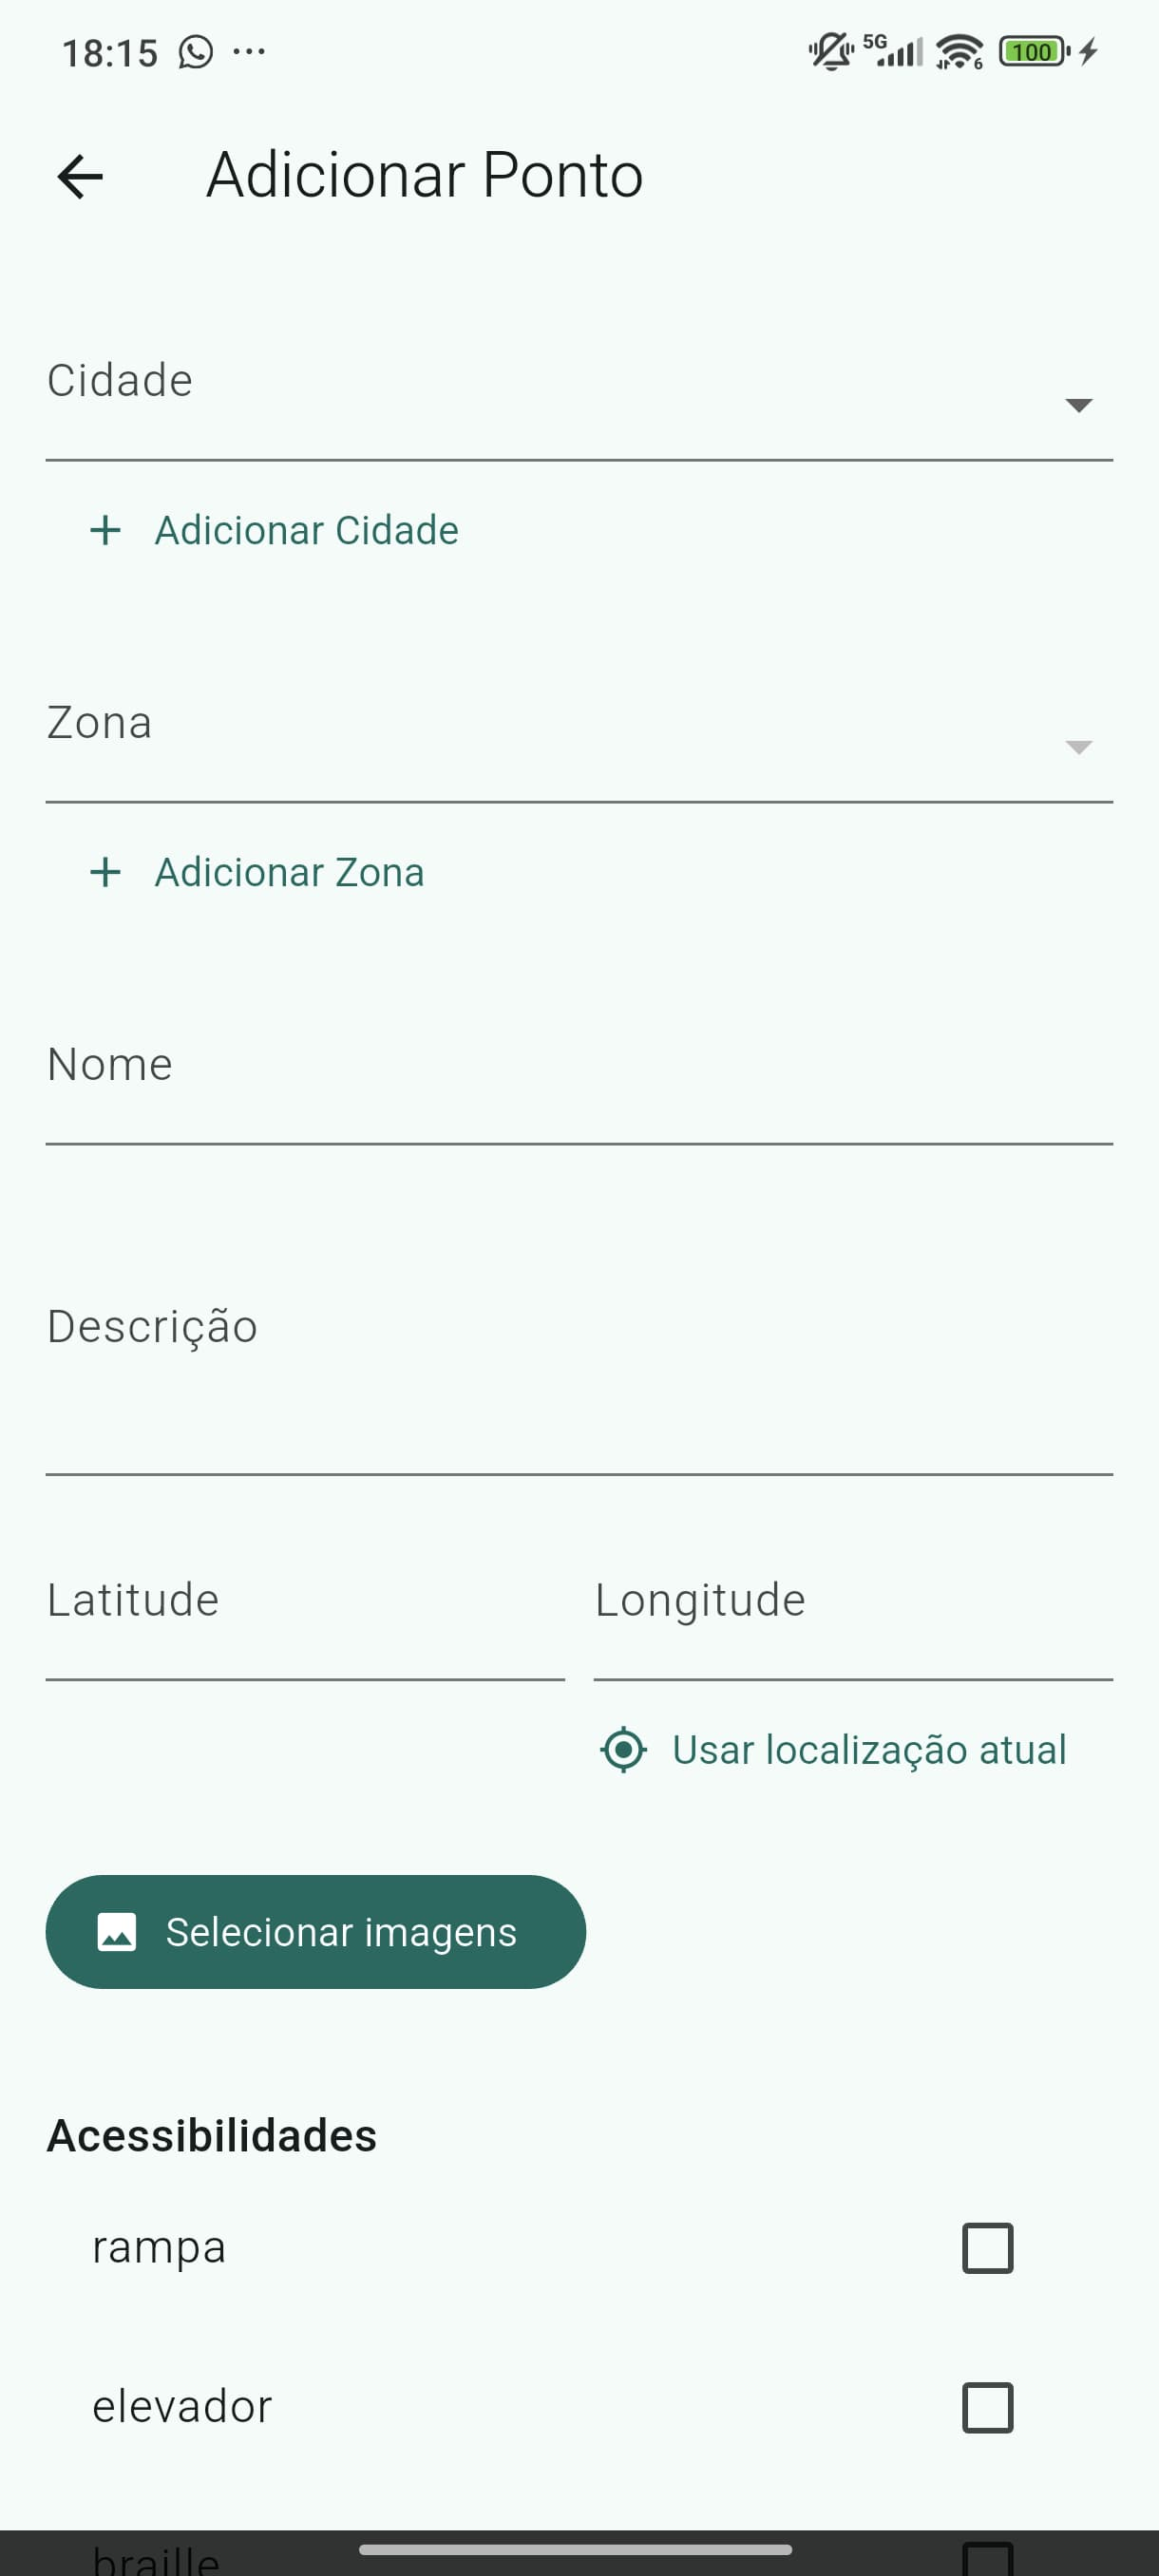
\includegraphics[scale=0.15]{imagens/adicionar_ponto.jpeg}
    \legend{Fonte: Elaborado pelo Autor}
\end{figure}

\begin{figure}[H]
	\caption{\label{fig:ss_ajudaai_06}Captura de Tela da Página de Adicinar Ponto - Adiconar Cidade}
    \centering
    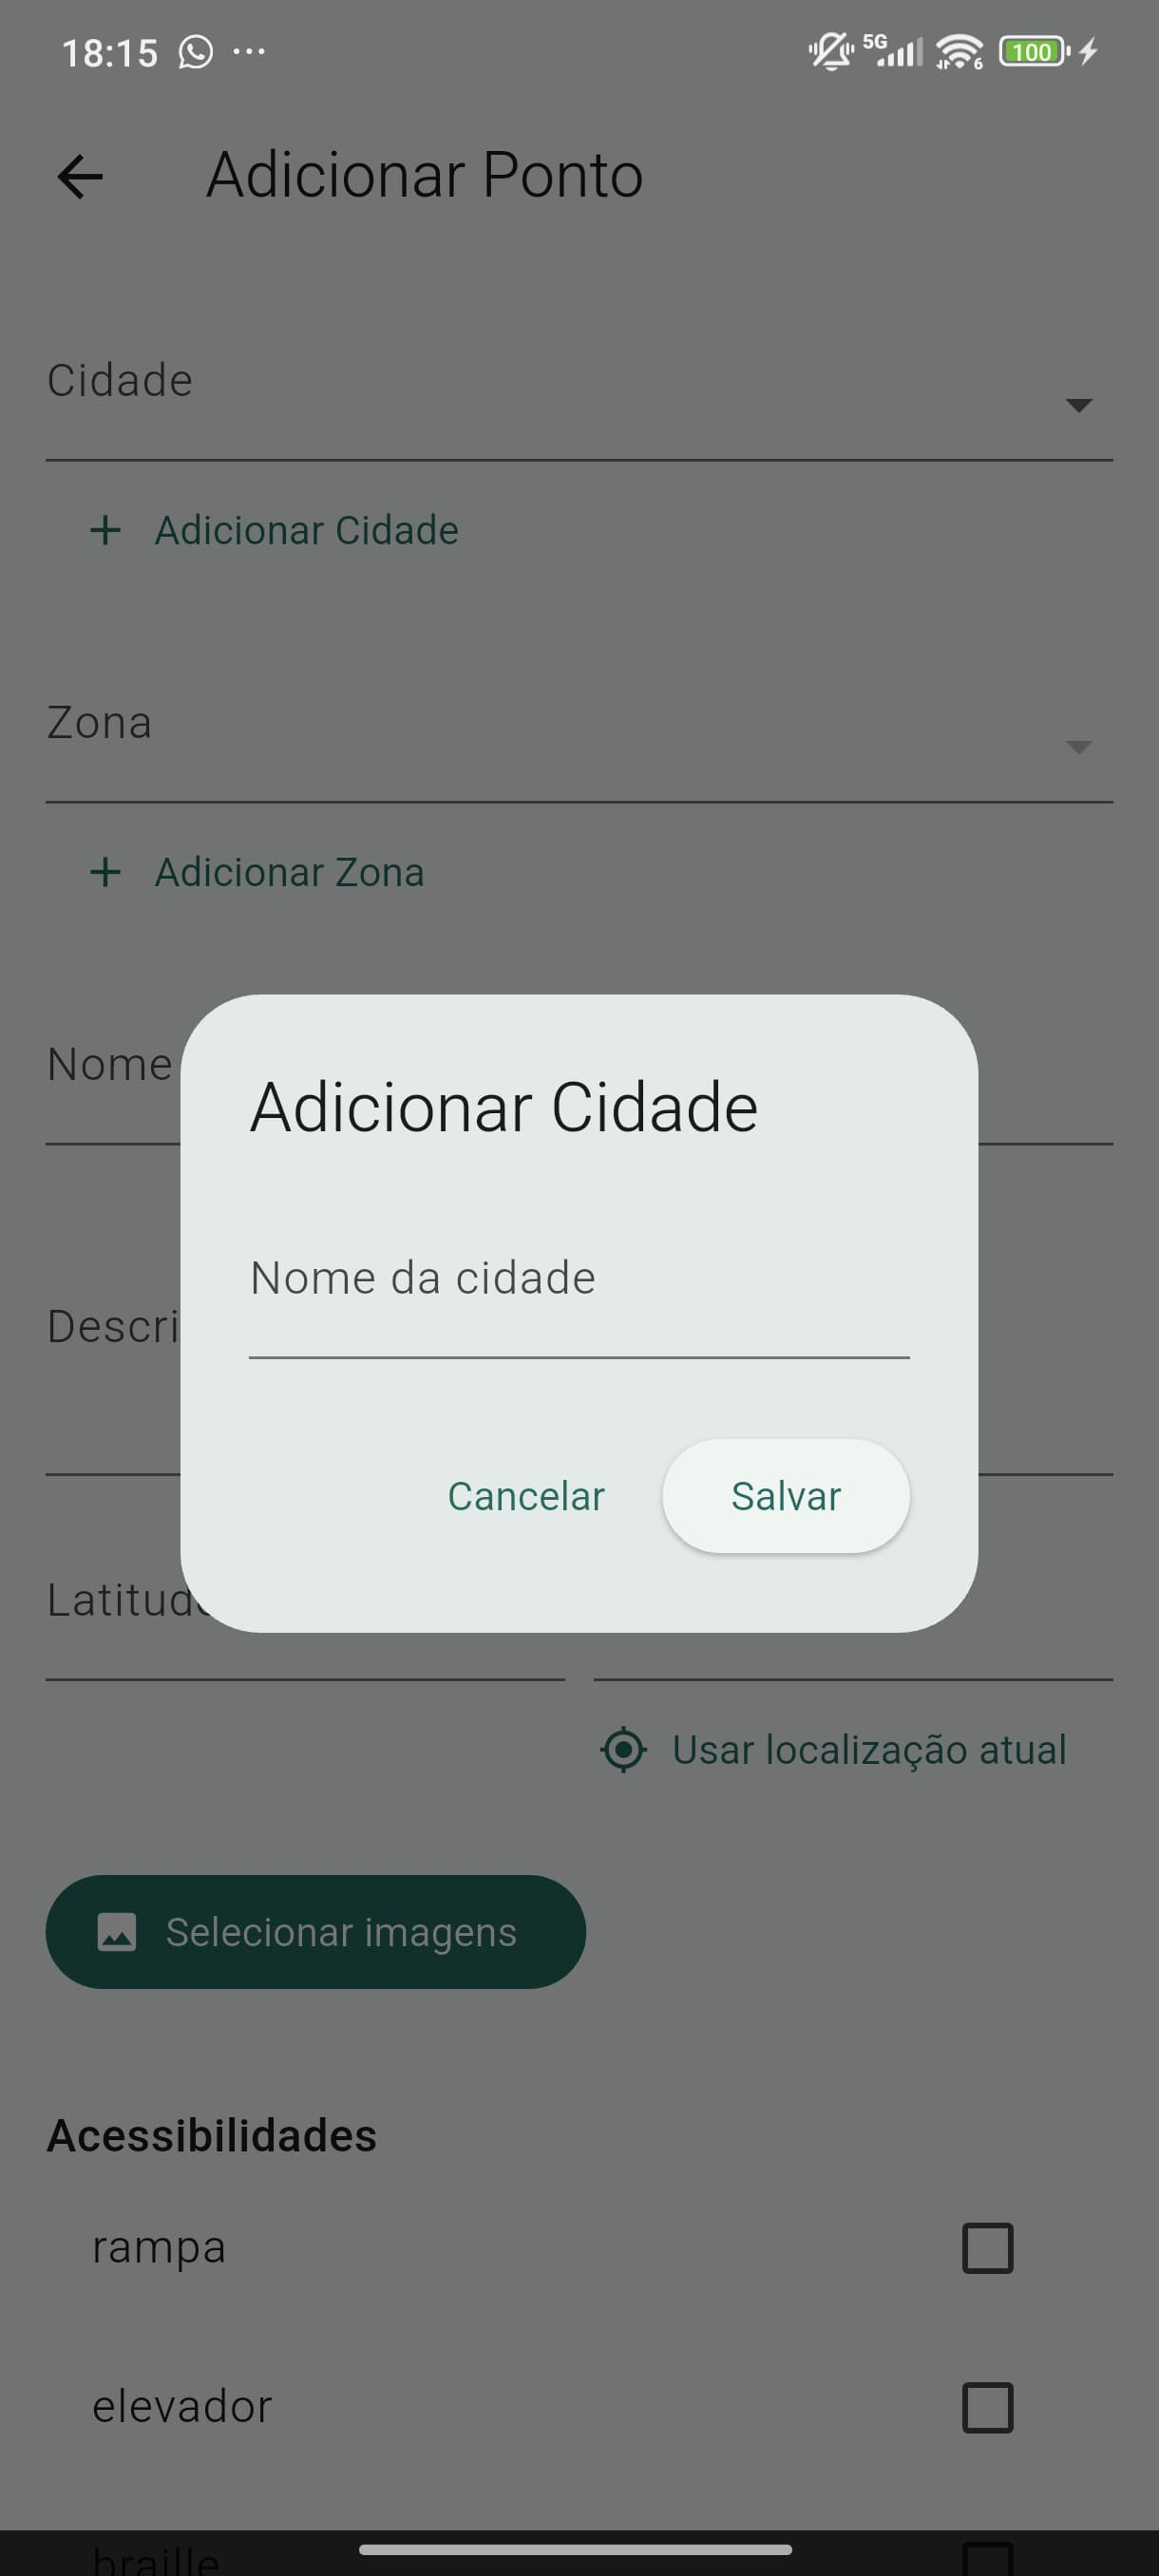
\includegraphics[scale=0.15]{imagens/adiconar_cidade.jpeg}
    \legend{Fonte: Elaborado pelo Autor}
\end{figure}

\begin{figure}[H]
	\caption{\label{fig:ss_ajudaai_07}Captura de Tela da Página de Adicinar Ponto - Adiconar Zona}
    \centering
    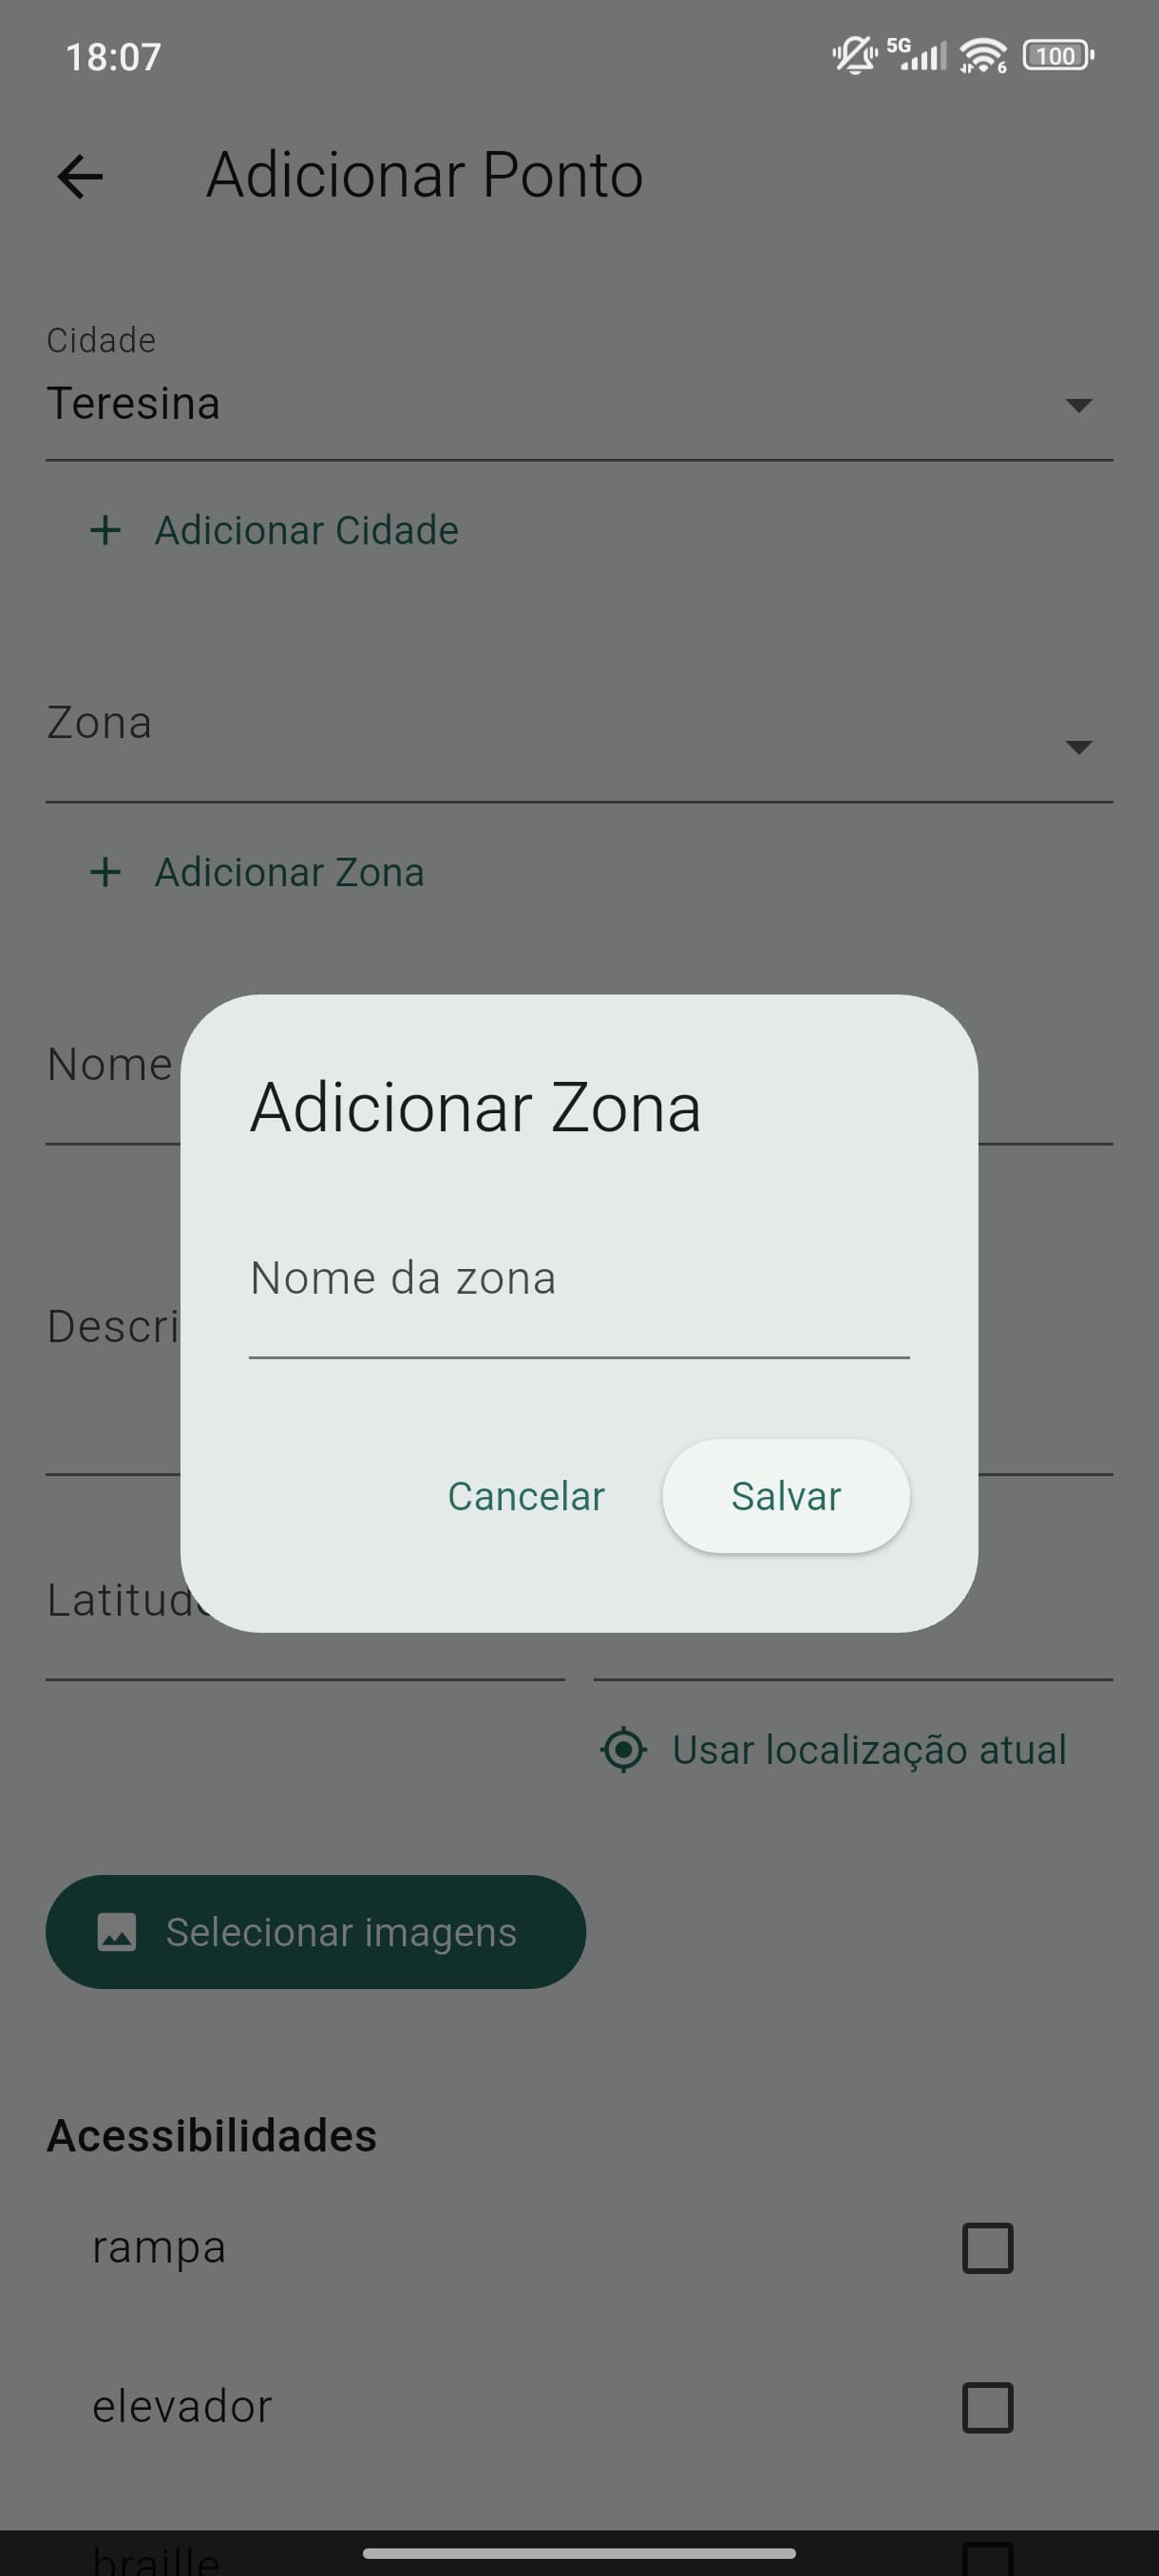
\includegraphics[scale=0.15]{imagens/adicionar_zona.jpeg}
    \legend{Fonte: Elaborado pelo Autor}
\end{figure}

Na tela de detalhes do ponto, são exibidas todas as informações cadastradas referentes ao local selecionado. Essa visualização inclui as imagens associadas ao ponto, a descrição fornecida no momento do cadastro e os tipos de acessibilidade disponíveis no local, como rampa de acesso, piso tátil, entre outros.

Essa tela foi desenvolvida com o objetivo de apresentar os dados de forma clara e organizada, permitindo que os usuários conheçam melhor o ponto cultural, suas características e as condições de acessibilidade oferecidas. Além disso, a disposição visual das informações busca garantir uma navegação intuitiva e uma boa experiência de uso.


\begin{figure}[H]
	\caption{\label{fig:ss_ajudaai_08}Captura de Tela de Detalhes do Ponto}
    \centering
    
\includegraphics[scale=0.15]{imagens/detalhes_ponto.jpeg}
    \legend{Fonte: Elaborado pelo Autor}
\end{figure}

\begin{figure}[H]
	\caption{\label{fig:ss_ajudaai_09}Captura de Tela de Detalhes do Ponto}
    \centering
    
\includegraphics[scale=0.15]{imagens/detalhes_ponto2.jpeg}
    \legend{Fonte: Elaborado pelo Autor}
\end{figure}




% \section{Organização do Projeto} \label{sec:ajudaai:organizacao}
% O projeto está organizado numa estrutura de Projeto Pai e Projetos Filhos do Apache Maven. Essa organização facilita na manutenção e montagem da aplicação no momento da distribuição ou \emph{deployment} da mesma. Os projetos filhos são:

% \begin{lista}
%   \item \textbf{util}: Classes utilitárias usado pelos outros projetos. As duas classes mais utilizadas são \codigo{StringUtils}, com utilitários para comparação e processamento de Strings, e \codigo{SendMail}, que utiliza a API \codigo{javax.mail} para enviar e-mails como HTML;
%   \item \textbf{model}: Contém o modelo de dados do Ajuda.Ai, apresentado na Figura \ref{fig:uml_model};
%   \item \textbf{persistence-sql}: Provê classes que implementam a persistência do projeto model em um banco de dados SQL através do JBoss Hibernate;
%   \item \textbf{backend}: Servidor de Back-end do Ajuda.Ai. Aplica as regras de negócio, organiza pagamentos e atende requisições dos usuários;
%   \item \textbf{frontend}: Aplicação de Página Única do Front-end do Ajuda.Ai;
%   \item \textbf{payment-api}: Projeto pai para as implementações de pagamentos dos diferentes \emph{Gateways} de pagamento;
%   \item \textbf{payment-impl-moip}: Implementação de payment-api para o \emph{gateway} MoIP;
%   \item \textbf{payment-impl-pagseguro}: Implementação de payment-api para o \emph{gateway} PagSeguro;
%   %\item \textbf{tests}: Testes do sistema.
% \end{lista}

% O modelo de dados da aplicação é apresentado na Figura \ref{fig:uml_model}, onde é apresentado um diagrama UML de classes do projeto \emph{model}. Estas são as principais entidades do sistema e seus relacionamentos:

% \begin{lista}
% %% ajuda.ai.model.user
% \item \codigo{\textbf{User}}: Usuário simples. Todos os usuários podem ter Instituições e só poderão alterar informações vinculadas a ele mesmo;

% %% ajuda.ai.model.extra
% \item \codigo{\textbf{CreationInfo}}: Entidade embarcável\footnote{Uma Entidade Embarcável é uma classe que, no esquema objeto-relacional da plataforma Java, não tem uma tabela no SGBD própria e sim faz parte da tabela das classes que se associam a esta classe.} que guarda quando uma entidade foi criada, que usuário a criou, quando foi feita a última alteração na entidade e qual usuário fez a alteração. Caso o usuário que criou ou alterou seja nulo se considera que foi uma ação tomada pelo próprio Sistema;
% \item \codigo{\textbf{Page}}: Uma página de conteúdo livre do Ajuda.Ai. Representa uma página web cujo conteúdo mude com pouca frequência;

% %% ajuda.ai.model.institution
% \item \codigo{\textbf{Institution}}: Representa uma Instituição criada por um Usuário;
% \item \codigo{\textbf{InstitutionPost}}: Uma página de conteúdo livre vinculada a uma Instituição. Estende \codigo{Page};

% %% ajuda.ai.model.billing
% \item \codigo{\textbf{Payment}}: Representa uma ordem de pagamento feita pelo Sistema a um \emph{Gateway} de Pagamento em nome de um Usuário;
% \item \codigo{\textbf{PaymentEvent}}: Representa uma mudança de estado de um pagamento como informado pelo \emph{Gateway} de Pagamento;
% \end{lista}

%As principais classes do sistema são \codigo{Instituion}, \codigo{Payment} e \codigo{PaymentEvent}. A primeira representa as Instituições cadastradas no sistema, as quais receberão doações de usuários, representados por \codigo{User}. Essas doações são representadas internamente como objetos \codigo{Payment} os quais abstraem de forma unificada pagamentos feitos através de diferentes \emph{Gateways} de Pagamento. Por fim, o andamento do pagamento junto ao \emph{Gateway} é informado através de notificações, como explicado em \ref{sec:ajudaai:processo_pagamento}, e essas notificações são, então, abstraídas como objetos \codigo{PaymentEvent} vinculados a um \codigo{Payment}.

% \begin{figure}[H]
% 	\caption{\label{fig:uml_model}Diagrama UML de Classes Resumido do Modelo do Ajuda.Ai}
%     \centering
% 	\begin{tikzpicture}
%     	\begin{umlpackage}[x=-3.5, y=0]{ajuda{.}ai{.}model{.}user}
%         	\umlclass[x=0, y=0]{User}{
%             	- id : Long \\
% 				- username : String \\
% 				- password : String \\
% 				- email : String \\
% 				- firstname : String \\
% 				- lastname : String
%             }{}
% 		\end{umlpackage}
        
%         \begin{umlpackage}[x=-1.5, y=-15.15]{ajuda{.}ai{.}model{.}billing}
%         	\umlclass[x=0, y=0]{Payment}{
%             	- id : Long \\
%                 - uuid : String \\
% 				- institution : Institution \\
%                 - creation : CreationInfo \\
% 				- description : String \\
% 				- paymentService : String \\
% 				- paymentServiceId : String \\
% 				- value : int \\
% 				- realValue : int \\
% 				- paid : boolean \\
% 				- readyForAccounting : boolean \\
% 				- cancelled : boolean \\
% 				- payeeName : String \\
% 				- payeeEmail : String \\
% 				- events : List<PaymentEvent>
%             }{}
%             \umlclass[x=7.5, y=0]{PaymentEvent}{
%             	- id : Long \\
%                 - payment : Payment \\
% 				- timestamp : Date \\
% 				- transactionServiceId : String \\
% 				- status : int \\
% 				- currency : String \\
% 				- value : int \\
% 				- paymentType : String \\
% 				- paymentTypeInfo : String
%             }{}
% 		\end{umlpackage}
        
%         \begin{umlpackage}[x=2.7, y=0]{ajuda{.}ai{.}model{.}extra}
%         	\umlclass[x=4.8, y=0]{Page}{
%             	- id : Long \\
% 				- slug : String \\
% 				- creation : CreationInfo \\
% 				- headerImage : String \\
% 				- title : String \\
% 				- subtitle : String \\
% 				- content : String \\
% 				- published : boolean
%             }{}
%             \umlclass[x=0, y=0]{CreationInfo}{
%             	- time : Date \\
% 				- lastUpdate : Date \\
% 				- creator : User \\
% 				- lastUpdateBy : User
%             }{}
% 		\end{umlpackage}
        
%         \begin{umlpackage}[x=-2.1, y=-6.45]{ajuda{.}ai{.}model{.}institution}
%         	\umlclass[x=0, y=0]{Institution}{
%             	- id : Long \\
% 				- slug : String \\
% 				- creation : CreationInfo \\
% 				- name : String \\
% 				- description : String \\
% 				- paymentService : String \\
% 				- attributes : Map<String, String>
%             }{}
%             \umlclass[x=6.5, y=0]{InstitutionPost}{
% 				- institution : Institution \\
% 				- pageviews : long
%             }{}
% 		\end{umlpackage}
        
        
		
        
        
%         \umlinherit[very thick]{InstitutionPost}{Page}
%         \umlcompo[arg1=*, arg2=1, very thick]{CreationInfo}{User}
%         \umlcompo[mult1=*, arg2=1, anchor1=65, very thick]{Payment}{Institution}
%         \umlcompo[arg1=1, arg2=*, very thick]{Payment}{PaymentEvent}
%         \umluniassoc[arg1=1, arg2=1, anchor1=58, anchor2=-120, very thick]{Payment}{CreationInfo}
%       	\umluniassoc[arg1=1, arg2=1, very thick]{Institution}{CreationInfo}
%         \umluniassoc[arg1=1, arg2=1, very thick]{Page}{CreationInfo}
%   \end{tikzpicture}
%   \legend{Fonte: Elaborado pelo Autor}
% \end{figure}

% As principais classes do sistema são \codigo{Instituion}, \codigo{Payment} e \codigo{PaymentEvent}. A primeira representa as Instituições cadastradas no sistema, as quais receberão doações de usuários, representados por \codigo{User}. Essas doações são representadas internamente como objetos \codigo{Payment} os quais abstraem de forma unificada pagamentos feitos através de diferentes \emph{Gateways} de Pagamento. Por fim, o andamento do pagamento junto ao \emph{Gateway} é informado através de notificações, como explicado em \ref{sec:ajudaai:processo_pagamento}, e essas notificações são então abstraídas como objetos \codigo{PaymentEvent} vinculados a um \codigo{Payment}.







% \section{Arquitetura} \label{sec:ajudaai:arquitetura}

% Como arquitetura do sistema se escolheu uma arquitetura REST Web onde o \emph{Back End} é totalmente separado do \emph{Front End}. Dessa forma, o \emph{Back End} preocupa-se apenas em atender requisições menores e que envolvem dados e regra de negócio e o \emph{Front End} preocupa-se apenas com a exibição de informações e a interação com o usuário. Assim, permite-se que seja feita uma separação completa entre \emph{Front End} e \emph{Back End} e a interface com o usuário pode ser feita se utilizando um navegador e HTML5 ou um aplicativo para plataformas móveis como Google Android e Apple iOS.

% A Figura \ref{fig:arquitetura} ilustra a arquitetura do Ajuda.Ai, que utiliza uma arquitetura REST Web, arquitetura recomendada para aplicações web pela W3C\footnote{\emph{World Wide Web Consortium}, consórcio de empresas e profissionais que buscam padronizar a WWW} em \cite{booth2004webservices}. Nessa especificação, REST Web é definido como um subconjuntos da WWW, baseado em HTTP, onde o servidor provê uma interface e semântica uniforme para as aplicações, sem impor uma interface específica. Além disso, todas as ações são tomadas através do que se chama de troca de representações de estado, ou seja, a entrada são objetos que representam uma requisição e a saída são objetos que representam uma resposta.

% \begin{figure}[H]
%   \caption{\label{fig:arquitetura}Arquitetura do Ajuda.Ai}
%   \centering
%   \includegraphics[scale=0.7]{imagens/ajudaAi-arquitetura.pdf}
%   \legend{Fonte: Elaborado pelo Autor}
% \end{figure}

% Requisições são feitas ao sistema de duas origens: A interface com o usuário e os \emph{gateways} de pagamento. As requisições feitas pela interface são padronizadas como JSON a fim de facilitar a criação de aplicações modernas e diminuir o tráfego de dados. Já requisições feitas pelos \emph{gateways} são suportadas em XML, JSON, \emph{x-www-form-urlencoded} (formulário HTML padrão) e \emph{form-data} (formulário HTML com dados longos, definido pelo RFC2388).

% Um dos diferenciais do Ajuda.Ai é o suporte a diferentes \emph{gateways} de pagamento. Isso dá flexibilidade a instituição para usar o \emph{gateway} mais adequado a mesma. Para implementação foi utilizado o Padrão de Projeto de Software \emph{Strategy}, como ilustrado na Figura \ref{fig:uml_strategy}. Este Padrão de Projeto é definido por uma família de algoritmos encapsulados e que podem ser trocados dentro da família de objetos \cite{gamma1995design}.

% \begin{figure}[H]
% 	\caption{\label{fig:uml_strategy}Estrutura dos Processadores de Pagamento}
%     \centering
% 	\begin{tikzpicture}
% 		\umlclass[type=interface]{PaymentGateway}{}{
% 			+ createPayment() : Payment \\
%             + processEvent() : PaymentEvent}
%         \umlclass[x=-3.5, y=-4]{MoipPaymentGateway}{}{
% 			+ createPayment() : Payment \\
%             + processEvent() : PaymentEvent}
%         \umlclass[x=3.5, y=-4]{PagSeguroPaymentGateway}{}{
% 			+ createPayment() : Payment \\
%             + processEvent() : PaymentEvent}
%         \umlsimpleclass[x=-3, y=3]{InstitutionController}
%         \umlsimpleclass[x=3, y=3]{TransactionNotificationController}
%         \umlcompo[very thick]{InstitutionController}{PaymentGateway}
%         \umlcompo[very thick]{TransactionNotificationController}{PaymentGateway}
%         \umlimpl[very thick]{MoipPaymentGateway}{PaymentGateway}
%         \umlimpl[very thick]{PagSeguroPaymentGateway}{PaymentGateway}
%   \end{tikzpicture}
%   \legend{Fonte: Elaborado pelo Autor}
% \end{figure}

% Cada implementação de \emph{gateway} de pagamento suportado implementa a interface \codigo{PaymentGateway}. Esta interface tem dois métodos:

% \begin{lista}
%   \item \textbf{\codigo{createPayment()}}: Cria uma ordem de pagamento junto ao \emph{gateway} de pagamento. Esse método tem liberdade de redirecionar o usuário para o sistema do \emph{gateway} (MoIP e a maioria dos gateways nacionais) ou enviar algum pedaço de informação, como JSON, como resposta ao usuário (PayPal + JavaScript para pagamento na própria página). Este método deve retornar um objeto \codigo{Payment} para ser persistido a fim de acompanhar o andamento do pagamento;

%   \item \textbf{\codigo{processPayment()}}: \emph{Gateways} de pagamento enviam requisições de volta ao sistema informando sobre o status de um determinado pagamento feito na plataforma deles. Esse método é encarregado de processar essas mudanças de estado no pagamento. Este método deve retornar um objeto \codigo{PaymentEvent} que indica de forma padronizada o que aconteceu com este pagamento.
% \end{lista}

% Ao criar uma ordem de pagamento através de \codigo{createPayment()} a classe que a criou retorna um objeto \codigo{Payment} para ser persistido. Esse objeto, além de padronizar as informações relevantes dos pagamentos, guarda consigo a estratégia (serviço de pagamento) utilizada para criar a ordem de pagamento. Essa informação é usada futuramente quando o sistema recebe uma notificação de estado de pagamento.

% Uma vantagem da utilização do padrão \emph{Strategy} é que diferentes usos de um mesmo \emph{gateway} podem ser facilmente implementados. Por exemplo, o \emph{gateway} MoIP oferece várias formas para criar ordens de pagamento. Três delas são interessantes para o que o Ajuda.Ai propõe:

% \begin{lista}
%   \item \textbf{Ordem de pagamento via e-mail:} O MoIP envia um e-mail para o usuário onde, na conveniência do mesmo, ele tem 30 dias para efetuar o pagamento da forma como preferir;
%   \item \textbf{\emph{Check-out} Clássico:} O usuário é redirecionado para o \emph{Gateway} onde ele selecionará forma de pagamento e fará todo o processo de pagamento antes de voltar ao Ajuda.Ai --- Essa forma está disponível em todos os \emph{gateways} e é a forma preferencial de se fazer a interação de pagamento junto ao usuário;
%   \item \textbf{\emph{Check-out} Transparente:} O usuário preenche tudo no próprio sistema o qual junto ao \emph{gateway} e através de \emph{webservices} faz uma ordem de pagamento e processamento de pagamento --- Esta forma está disponível em quase todos os \emph{gateways}.
% \end{lista}

% O Ajuda.Ai se utiliza da segunda forma demonstrada, o \emph{Check-Out} Clássico, pois é suportada por todos os \emph{gateways} e recomendada pelos mesmos por prover um ambiente seguro e que os usuários demonstram maior confiança ao partilhar dados sigilosos e pessoais como números de cartão de crédito e CPF. Esse processo de pagamento será detalhado na próxima subseção.





% \subsection{Processo Comum de Pagamentos Online} \label{sec:ajudaai:processo_pagamento}

% A ilustração da Figura \ref{fig:gateway} mostra o fluxo de criação e processamento de pagamento comum a maioria dos \emph{gateways} atualmente no mercado. Todo o processo acontece entre duas entidades que são o Sistema, que é o sistema que irá gerar as ordens de pagamento e ser notificado do andamento dos pagamentos, e o próprio \emph{Gateway} de Pagamento. O processo começa com a geração de uma ordem de pagamento junto ao \emph{gateway}, a qual pode ser feita de duas maneiras:

% \begin{lista}
% 	\item \textbf{Pagamento Normal}: Nessa modalidade, o Sistema faz um HTTP POST com dados sobre o que está sendo comprado ao \emph{Gateway} e o usuário é redirecionado até uma página do próprio \emph{Gateway} de pagamento. Esse é o modo recomendado pelos \emph{Gateways}, pois os \emph{Gateways} podem servir a página de forma segura, protegida através de certificados digitais confiáveis, com uma interface de usuário adequada. Segundo os \emph{Gateways}, os clientes ficam mais propensos a concluir a compra quando o pagamento utiliza esse formato, pois os mesmos confiam na marca do \emph{Gateway} e na segurança do ambiente;
% 	\item \textbf{Pagamento Transparente}: Nessa modalidade, todos os dados do pagamento são preenchidos em uma interface provida pelo próprio Sistema e enviados de forma segura ao \emph{Gateway} de Pagamento, o qual imediatamente cria e inicia o processamento do pagamento da uma ordem de pagamento.
% \end{lista}

% \begin{figure}[H]
% 	\caption{\label{fig:gateway}Fluxo de um Pagamento via \emph{Gateway} de Pagamento}
%     \centering
%     \includegraphics[scale=0.575]{imagens/processo_gateway.pdf}
%     \legend{Fonte: Elaborado pelo Autor}
% \end{figure}

% O Ajuda.Ai faz uso da primeira maneira, o Pagamento Normal, onde o usuário é redirecionado ao \emph{Gateway}. Após a criação do pedido de pagamento e o preenchimento das informações necessárias, como dados pessoais, CPF e outros, o \emph{Gateway} cria um pagamento em seu sistema, e a partir desse ponto começa a máquina de estados do \emph{Gateway}. A máquina apresentada é uma simplificação e normalização do que ocorre na maioria dos \emph{Gateways}.

% Na ilustração da Figura \ref{fig:gateway} as setas de cor azul representam o fluxo como visto pelo usuário do Sistema. O usuário preenche algumas informações no próprio Sistema ou no \emph{Gateway} e, ao enviar, é feita a ordem de pagamento e o usuário é redirecionado de volta ao Sistema em uma página de ``Obrigado''. Esta é uma página do Sistema para onde o \emph{Gateway} irá redirecionar o usuário ao final do fluxo de criação da ordem de pagamento.

% Ao criar uma ordem de pagamento, inicia-se uma máquina de estados do pagamento que muda de acordo com o andamento do pagamento ou ações do usuário. Durante os estados na máquina de estados do \emph{Gateway} cada alteração de estado resulta em uma notificação ao sistema, representadas pelas setas na cor laranja. Esse comportamento é típico do padrão de projetos \emph{Event Notifier}, também conhecido como \emph{Publish-Subscribe} ou \emph{Pub-Sub}. Esse padrão de projeto permite que dois sistemas comuniquem eventos entre si sem necessariamente ter conhecimento um do outro \cite{gupta2000event}.

% Como parte da implementação deste padrão de projeto, os \emph{gateways} de pagamento provêm alguma maneira de configurar quais URL do Sistema deverá ser chamada para receber as notificações geradas pelas trocas de estado. Na ilustração da Figura \ref{fig:config_moip} está a configuração desta opção no sistema do \emph{gateway} MoIP.

% \begin{figure}[H]
% 	\caption{\label{fig:config_moip}Configuração de Notificação do \emph{Gateway} de Pagamento MoIP}
%     \centering
%     \includegraphics[scale=0.85]{imagens/config-moip.png}
%     \legend{Fonte: Elaborado pelo Autor}
% \end{figure}

% A cada alteração de estado do pagamento uma requisição específica a URL configurada será feita. Para facilitar a configuração dos vários diferentes \emph{gateways} no mercado a URL do Ajuda.Ai a ser configurada neles é padronizada, mudando apenas um parâmetro que representa qual \emph{gateway} fará requisições a URL. Na ilustração da Figura \ref{fig:config_moip} temos a URL referente ao MoIP.

% Uma vez criado um pagamento junto ao \emph{gateway} ele deve ser confirmado. Esse estado é mais evidente quando o pagamento é feito por Boleto Bancário, pois o mesmo demora até 3 dias úteis para ser processado pelo banco e o retorno dado ao \emph{gateway}. Em pagamentos via cartão de crédito a confirmação é simplesmente o recebimento da requisição de crédito através dos sistemas da mesma, o que quase sempre é imediato.

% Na confirmação o \emph{gateway} é informado do sucesso ou falha na execução do pagamento. Caso o pagamento tenha sido feito sem problemas, ele vai para o estado Finalizado, vai para Recusado. Como explicitado na Figura \ref{fig:gateway}, a praticamente qualquer momento do processo o usuário poderá Cancelar o pagamento. Apenas após 30 dias no estado Finalizado, o cancelamento da operação fica indisponível, entretanto este prazo pode mudar de acordo com o \emph{gateway}. Vale salientar também, que apenas após este prazo o dinheiro estará disponível para resgate pela instituição.

% Cada mudança de estado resulta em uma chamada a URL configurada juntamente a um pacote de informações sobre o estado atual do pagamento. Cada \emph{Gateway} envia informações distintas, mas bastante semelhantes. A mais importante delas é o que é chamado de ID do Cliente que é um número especificado pelo Sistema e que será vinculado aquele pagamento. Este campo deve ser utilizado pelo Sistema para identificar internamente o que está sendo pago. O Ajuda.Ai utiliza este campo para manter o ID do objeto \codigo{Payment} gerado no início do processo a fim de manter o estado do pagamento e vincular a instituição correspondente.





% \section{API REST Web} \label{sec:ajudaai:api}

% Para facilitar o desenvolvimento de diferentes interfaces com o usuário e demais consumidores da API e prevenir dúvidas quanto a mesma e seu funcionamento a API REST Web do \emph{backend} do projeto Ajuda.Ai foi documentada. Esses são os métodos da API que estão disponíveis para todos os clientes, porém alguns necessitam de login. Os métodos que não necessitam de login são classificados como métodos públicos.

% Apesar da importância de uma boa documentação ainda não há um padrão estabelecido para a forma de documentar APIs REST Web. Por esse motivo este trabalho se utiliza do formato proposto por Irene Ros\cite{blog:bocoup}, diretora da Bocoup, empresa de consultoria referência em desenvolvimento REST Web e produtora de diversas ferramentas de código fonte aberto para se trabalhar com REST Web e \emph{Front-end}. No anexo \ref{anexo:a}, encontra-se documentada a API REST Web disponibilizada pelo Ajuda.Ai.





\section*{Resumo} \label{sec:ajudaai:resumo}
Neste capítulo, foi apresentado o protótipo da solução proposta, representado pelo aplicativo de registro de pontos culturais. Foram descritas suas principais funcionalidades, incluindo a navegação pelas telas, os recursos de cadastro, visualização, filtros de busca e acessibilidade. O protótipo ilustra como a aplicação pretende contribuir para o mapeamento e a valorização da cultura local, oferecendo uma ferramenta tecnológica acessível e funcional.

No capítulo seguinte, temos a Conclusão do trabalho, dado seus objetivos propostos além do cronograma de atividades do trabalho.